%%%%%%%%%%%%%%%%%%%%%%%%%%%%%%%%%%%%%%%%%%%%%%%%%%%%%%%%%%%%%%%%%%%%%%%
%
% CC BY-NC-SA 4.0
%
% Template für die Erstellung einer Abschlussarbeit an der TH Nürnberg
% Author: Prof. Dr. Christine Niebler, TH Nürnberg
% Überarbeitung: Hannes Dippold, Fachschaft EFI
%
% Das Template muss mit pdflatex und biber kompiliert werden
% Für Fragen stehe ich gerne zur Verfügung
%
%
%%%%%%%%%%%%%%%%%%%%%%%%%%%%%%%%%%%%%%%%%%%%%%%%%%%%%%%%%%%%%%%%%%%%%%%

% Definition des Dokumentenlayouts
% parskip=half wurde entfernt, da wir klassischen Absatzeinzug verwenden möchten.
\documentclass[
  a4paper,
  titlepage=yes,
  11pt,
  BCOR=12mm
]{scrreprt}

% Einbinden der Präambel
%!TeX root=00_Abschlussarbeit.tex
% \pdfcompresslevel=0
% \pdfobjcompresslevel=0

% Pakete für die Darstellung und Eingabemöglichkeit von Umlauten
\usepackage[T1]{fontenc}
\usepackage[utf8]{inputenc}
\usepackage{lmodern}
% \usepackage{fontspec}   ← auskommentiert lassen
% \setmainfont{...}       ← auskommentiert lassen


%Für Tabellen
\usepackage{rotating}   % Drehen
\usepackage{colortbl}   % Farben
\usepackage{booktabs}   % dickere Linien
\usepackage{longtable}  % für lange Tabellen
\usepackage{tabularx}
\usepackage{array}
\usepackage{multirow}
\usepackage{diagbox}    % für diagonale Linien in Tabellen
\usepackage{float}      % für Tabellenpositionierung [H]
\usepackage{xcolor, colortbl}
\usepackage{caption}    % für \captionof
\usepackage{array}
\newcolumntype{L}[1]{>{\raggedright\arraybackslash}p{#1}}
\newcolumntype{C}[1]{>{\centering\arraybackslash}p{#1}}




% Benötigte Pakete in der Präambel:
 \usepackage{booktabs}
 \usepackage{array}
 \usepackage{colortbl}
 \usepackage[table]{xcolor}
 \usepackage{graphicx}
 \usepackage{diagbox}
 \usepackage{threeparttable}


% Anpassung Seitenränder
\usepackage[left= 3cm, right = 2cm, bottom = 3 cm, top = 2cm]{geometry} 

% Verwendung deutscher Begriffe für automatisch generierte Worte wie z.B. "Inhaltsverzeichnis"
\usepackage[ngerman, english]{babel}

% Anführungszeichen/Zitate
\usepackage{csquotes}

% Trennen wenn Latex es nicht richtig macht:
% \hyphenation{}

% Paket um Dummy-Text/Blindtext zu erzeugen
\usepackage{blindtext}

% Eigenes Titelblatt
\usepackage{LTXKursTitel}

% Zeilenabstand auf 1,5 setzen
\usepackage[onehalfspacing]{setspace}
    \AfterTOCHead{\singlespacing}
    %\KOMAoptions{DIV=last}          % KOMA Klasse für europ. Layout
\usepackage{scrdate, scrtime}       % Zeit und Datumsbefehle
\usepackage{scrlayer-scrpage}       % Erweitere Layout-Optionen
    \pagestyle{scrheadings}         % Seitenlayout selbst definieren

% Belegung von KOMA Variablen für Kopf- und Fußzeilen Gestaltung
    \newcommand{\footlinetext}{\footnotesize \textsf{\color{gray} Kapitel \thesection \  \normalsize}}
    \KOMAoptions{headsepline = yes, footsepline = no}
    \ihead{}
    \chead{Kapitel \thesection}
    \ohead{}
    \ifoot{}
    \cfoot{\pagemark}
    \ofoot{}

% Pakete zum Einbinden von Bildern und Farben
\usepackage{xcolor}
\definecolor{chapterblue}{RGB}{0,70,140}
\setkomafont{chapter}{\color{chapterblue}\huge\sffamily\bfseries}
\setkomafont{section}{\color{chapterblue}\Large\sffamily\bfseries}
\setkomafont{subsection}{\color{chapterblue}\large\sffamily\bfseries}
\setkomafont{subsubsection}{\color{chapterblue}\large\sffamily\bfseries}

 

\usepackage{graphicx}
\usepackage{pdfpages} %PDFs einbinden


% Pakete für Mathematik
\usepackage[free-standing-units,locale = DE]{siunitx}   % Befehle für SI-Einheiten
\usepackage{amsmath}                                    % Mathematik Befehle
\usepackage{amsfonts}

% Paket und Spezifikation der Parameter zur Darstellung von Programmcode mit Courier-Schriftart
\usepackage{listings}  % Darstellung von Quellcode
\usepackage{courier}   % Schriftart laden
    \lstset{
    language=Python,                % Programmiersprache
    basicstyle=\footnotesize\ttfamily,  % Standardschrift
    numbers=left,                       % Ort der Zeilennummern
    numberstyle=\tiny,                  % Stil der Zeilennummern
    %stepnumber=2,  % Abstand zwischen den Zeilennummern
    numbersep=5pt,  % Abstand der Nummern zum Text
    tabsize=2,      % Groesse von Tabs
    extendedchars=true, %
    breaklines=true,    % Zeilen werden Umgebrochen
    keywordstyle=\color{blue}\bfseries,
    frame=b,
    % keywordstyle=[1]\textbf, % Stil der Keywords
    % keywordstyle=[2]\textbf, %
    % keywordstyle=[3]\textbf, %
    % keywordstyle=[4]\textbf, \sqrt{\sqrt{}} %
    stringstyle=\color{magenta}\ttfamily, % Farbe der String
    showspaces=false,   % Leerzeichen anzeigen ?
    showtabs=false,     % Tabs anzeigen ?
    %xleftmargin=17pt,  % Abstände
    %framexleftmargin=17pt,
    %framexrightmargin=5pt,
    %framexbottommargin=4pt,
    commentstyle=\color{gray},
    %backgroundcolor=\color{grey},
    showstringspaces=false,      % Leerzeichen in Strings anzeigen ?
    morekeywords={__global__},  % additional language specific keywords
    morecomment=[l]
    }
    \lstloadlanguages{% Check Dokumentation for further languages ...
    %[Visual]Basic
    %Pascal
    C,
    C++,
    %XML
    %HTML
    %Matlab
    %Java
    }

% Pfade und Topics umbrechbar darstellen
\usepackage{url}
\newcommand{\topic}[1]{\path{#1}}


% Literaturverzeichnis mit BibLaTeX und Biber erstellen
\usepackage[style=ieee, sorting=none, backend=biber]{biblatex}
% bib-Datei einbinden
\addbibresource{Literatur.bib}

\usepackage{abstract}

\usepackage[printonlyused]{acronym} %Abkürzungsverzeichnis

\usepackage{tocbasic}
\usepackage{textcmds}
\usepackage{scrhack}    %gets rid of \float@addtolists error

\allowdisplaybreaks[2]


\usepackage{enumitem}
\setlist{itemsep=0.05\baselineskip, leftmargin=1.4cm}

% Punkte im Inhaltsverzeichnis einfügen (mit tocbasic)

% Punkte ins Inhaltsverzeichnis
\DeclareTOCStyleEntry[beforeskip=5pt, entryformat=\normalfont, pagenumberformat=\normalsize, linefill=\dotfill]{chapter}{chapter}
\DeclareTOCStyleEntry[beforeskip=5pt, indent=1.5em, pagenumberformat=\normalsize, linefill=\dotfill]{tocline}{section}
\DeclareTOCStyleEntry[beforeskip=5pt, indent=3.8em, pagenumberformat=\normalsize, linefill=\dotfill]{tocline}{subsection}




\usepackage{hyperref}   % Layout im PDF Viewer. Muss als letztes Paket geladen werden
    \hypersetup{%
    plainpages=false,
    linktocpage=false,%true,
    breaklinks=true,
    colorlinks=true,
    linkcolor=black,%blue,
    anchorcolor=black,
    citecolor=black,%green,
    filecolor=black,%blue,
    urlcolor=black,%blue%
    pdfstartview={FitV},
    pdfview={FitH},
    pdfpagelayout={SinglePage},
    %pdfpagemode={None},   %unknown value "None"
    }

\usepackage[xindy, order=letter, acronym=true, toc]{glossaries} % muss nach hyperref geladen werden
% \usepackage{glossaries-german} % verwendete Sprachen laden, https://www.ctan.org/pkg/glossaries-german, nötig?

% Zusätzliches Symbolverzeichnis definieren, wichtig vor \makeglossaries
\newglossary[slg]{symbols}{syi}{syg}{Symbolverzeichnis}


\makeglossaries

% Stil definieren (dein eigener Stil)
% Wichtig: description-Umgebung braucht \item, sonst kommt "missing \item".
\usepackage{longtable}

% Zuordnung der Buchstaben-Gruppen (aus den sort-Schlüsseln in 04_Symbole.tex)
% zu den Kategorieüberschriften des Symbolverzeichnisses.
% Unbekannte Buchstaben werden unverändert ausgegeben (Fallback).
\makeatletter
\newcommand*{\symgroupname}[1]{%
  \ifcsname symgrp@#1\endcsname\csname symgrp@#1\endcsname\else#1\fi
}
\@namedef{symgrp@A}{Typografische Konvention}
\@namedef{symgrp@B}{Koordinatensysteme und Frames}
\@namedef{symgrp@C}{Orientierungsdarstellung}
\@namedef{symgrp@D}{Koordinatentransformationen}
\@namedef{symgrp@E}{Extrinsische Kalibrierung}
\@namedef{symgrp@F}{Kamera-Kalibrierung}
\@namedef{symgrp@G}{Extended Kalman Filter}
\@namedef{symgrp@H}{Faktorgraph-Optimierung}
\@namedef{symgrp@I}{Posenberechnung je Marker}
\@namedef{symgrp@J}{Kartenunsicherheit in der Gewichtung}
\@namedef{symgrp@K}{Ausreißerfilterung mit RANSAC}
\@namedef{symgrp@L}{Kamerafusion und Glättung}
\@namedef{symgrp@M}{Kovarianzschätzung}
\@namedef{symgrp@N}{Dead-Reckoning-Lokalisierung}
\makeatother

% Kompakter, tabellenartiger Stil für das Symbolverzeichnis
\newglossarystyle{symstyle}{
  \renewenvironment{theglossary}
    {\begin{longtable}{@{}p{1.3cm}p{\dimexpr\linewidth-1.6cm\relax}@{}}} % Abstand zwischen Symbol und Beschreibung
    {\end{longtable}}

  \renewcommand*{\glossentry}[2]{%
    \glstarget{##1}{\glossentryname{##1}} &
    \glossentrydesc{##1} \\[0.3em] % Abstand zwischen Einträgen
  }

  \renewcommand*{\subglossentry}[3]{%
    \glossentry{##2}{##3}%
  }

  % Benannte Kategorieüberschriften (Titel via \symgroupname aus dem Gruppen-Buchstaben)
  \renewcommand*{\glsgroupheading}[1]{%
    \multicolumn{2}{@{}l}{%
      \rule{0pt}{4.2ex}%
      \normalfont\sffamily\bfseries\large\color{chapterblue}\symgroupname{##1}%
    }\\[0.5em]%
  }
  \renewcommand*{\glsgroupskip}{}
}


% Eigener Stil für das Abkürzungsverzeichnis
\newglossarystyle{acronymstyle}{
  \renewenvironment{theglossary}
    {\begin{longtable}{@{}p{3cm}p{\dimexpr\linewidth-3cm\relax}@{}}}
    {\end{longtable}}

  \renewcommand*{\glossentry}[2]{%
    \glstarget{##1}{\glossentryname{##1}} &
    \glossentrydesc{##1} \\[0.3em] % Abstand zwischen Einträgen
  }

  \renewcommand*{\subglossentry}[3]{%
    \glossentry{##2}{##3}%
  }

  \renewcommand*{\glsgroupheading}[1]{}
  \renewcommand*{\glsgroupskip}{}
}


\setacronymstyle{long-short}
\setglossarystyle{list} %alternativ: tree, list, long3col, index weitere: https://www.dickimaw-books.com/gallery/glossaries-styles/#long

\setcounter{tocdepth}{4} %Erweiterung des Inhaltsverzeichnisses um eine weitere Ebene
\setcounter{secnumdepth}{4} %Erweiterung der Kapiteltiefe um eine weitere Ebene


\renewcommand{\familydefault}{\sfdefault}
%\usepackage{showframe}

% Kopfzeilen-Abstand reduzieren
\setlength{\headheight}{14pt}
\setlength{\headsep}{10pt}
 
% Kapitel oben beginnen lassen
\RedeclareSectionCommand[
  beforeskip=0pt,
  afterskip=1\baselineskip
]{chapter}
 
\RedeclareSectionCommand[
  beforeskip=1.5ex plus 0.5ex minus 0.2ex,
  afterskip=0.5ex
]{section}
 
\RedeclareSectionCommand[
  beforeskip=1ex plus 0.5ex minus 0.2ex,
  afterskip=0.5ex
]{subsection}

 
 
% Abstract nicht mittig
\setlength{\absleftindent}{0pt}
\setlength{\absrightindent}{0pt}
\setlength{\abstitleskip}{0pt}


% Einheitliche Abstände um abgesetzte Gleichungen
\AtBeginDocument{%
  \setlength{\abovedisplayskip}{0.7\baselineskip}
  \setlength{\belowdisplayskip}{0.7\baselineskip}
  \setlength{\abovedisplayshortskip}{0.7\baselineskip}
  \setlength{\belowdisplayshortskip}{0.7\baselineskip}
}


%%%%%%%%%%%%%%%%%%%%%%%%%%%%%%%%%%%%%%%%%%%%%%%%%%%
%%%          Variablen zum Belegen              %%%
%%%%%%%%%%%%%%%%%%%%%%%%%%%%%%%%%%%%%%%%%%%%%%%%%%%

% Variables for title page
    \DAAutor{\par Hannes Müller\par 3796115}
    \DATyp{}
    \DAAutorAdresse{Masterarbeit im Studiengang Elektronische und Mechatronische Systeme\par Vertiefungsrichtung Automatisierungstechnik}
    \DAFachbereich{Elektrotechnik Feinwerktechnik Informationstechnik}
    \DATitel{Implementierung eines fiducialbasierten Lokalisierungssystems für Luftfahrzeuge im Innenraum}
    \DABetreuerTextA{Betreuer}
    \DABetreuerTextB{Betreuer}
    \DABetreuerA{Prof. Dr. rer. nat. Pfitzner}
    \DABetreuerB{Prof. Dr.-Ing. Schröder}
    \DAOrt{Abgabe: Nürnberg}
    \DAAbgabedatum{??.\,Juli 2026}
    \DAAbgabesemester{Sommersemester 2026}

% Römische Seitenzahlen für Verzeichnisse/Vorspann
\pagenumbering{Roman}

% Pakete
\usepackage{placeins}

% hyperref möglichst spät laden
\usepackage{hyperref}
\usepackage[ngerman,noabbrev]{cleveref}


\crefname{figure}{Abbildung}{Abbildungen}
\Crefname{figure}{Abbildung}{Abbildungen}

\crefname{table}{Tabelle}{Tabellen}
\Crefname{table}{Tabelle}{Tabellen}

\crefname{section}{Abschnitt}{Abschnitte}
\Crefname{section}{Abschnitt}{Abschnitte}

\crefname{equation}{Gleichung}{Gleichungen}
\Crefname{equation}{Gleichung}{Gleichungen}

% Einstellungen für Quellcode

\renewcommand*{\lstlistingname}{Quellcode}

\lstset{
    aboveskip=1.0\baselineskip,
    belowskip=1.0\baselineskip,
    numbers=left,
    xleftmargin=10pt,
    inputencoding=utf8,
    extendedchars=true,
    literate=
        {ä}{{\"a}}1
        {ö}{{\"o}}1
        {ü}{{\"u}}1
        {Ä}{{\"A}}1
        {Ö}{{\"O}}1
        {Ü}{{\"U}}1
        {ß}{{\ss}}1
}



% -------------------------------------------------
% Absatzformatierung
% -------------------------------------------------

\setlength{\parindent}{15pt}
\setlength{\parskip}{0pt}

\usepackage{etoolbox}

% Erster Absatz nach Überschriften NICHT einrücken
\RedeclareSectionCommand[afterindent=false]{chapter}
\RedeclareSectionCommand[afterindent=false]{section}
\RedeclareSectionCommand[afterindent=false]{subsection}
\RedeclareSectionCommand[afterindent=false]{subsubsection}

% Erster Absatz nach Abbildungen/Tabellen NICHT einrücken
\usepackage{noindentafter}

\NoIndentAfterEnv{figure}
\NoIndentAfterEnv{table}
\NoIndentAfterEnv{equation}
\NoIndentAfterEnv{gather}
\NoIndentAfterEnv{align}
\NoIndentAfterEnv{verbatim}
\NoIndentAfterEnv{lstlisting}
\NoIndentAfterEnv{itemize}
\NoIndentAfterEnv{enumerate}

% \FloatBarrier so erweitern, dass danach kein Einzug kommt
% Originalen FloatBarrier-Befehl sichern
\makeatletter
\let\OldFloatBarrier\FloatBarrier

\renewcommand{\FloatBarrier}{%
  \OldFloatBarrier
  \@afterindentfalse
  \@afterheading
}
\makeatother


% Wichtig:
% \usepackage{indentfirst} NICHT verwenden,
% damit der erste Absatz nach einer Überschrift nicht eingerückt wird.

% -------------------------------------------------
% Abstände vor und nach Überschriften
% KOMA-Script: scrreprt
% -------------------------------------------------

% Kapitelüberschriften
\RedeclareSectionCommand[
  beforeskip=0pt,
  afterskip=1.1\baselineskip
]{chapter}

% Abschnittsüberschriften
\RedeclareSectionCommand[
  beforeskip=1.1\baselineskip,
  afterskip=0.7\baselineskip
]{section}

% Unterabschnittsüberschriften
\RedeclareSectionCommand[
  beforeskip=1.0\baselineskip,
  afterskip=0.7\baselineskip
]{subsection}

% Unterunterabschnittsüberschriften
\RedeclareSectionCommand[
  beforeskip=0.8\baselineskip,
  afterskip=0.5\baselineskip
]{subsubsection}

%% Hier startet der Dokumenteninhalt
\begin{document}

\thispagestyle{empty}
\null
\newpage

% Deckblatt einbinden
\maketitle

% Eigenständigkeitserklärung einbinden,
% auskommentiert lassen, solange noch nicht existent
\begin{center}
  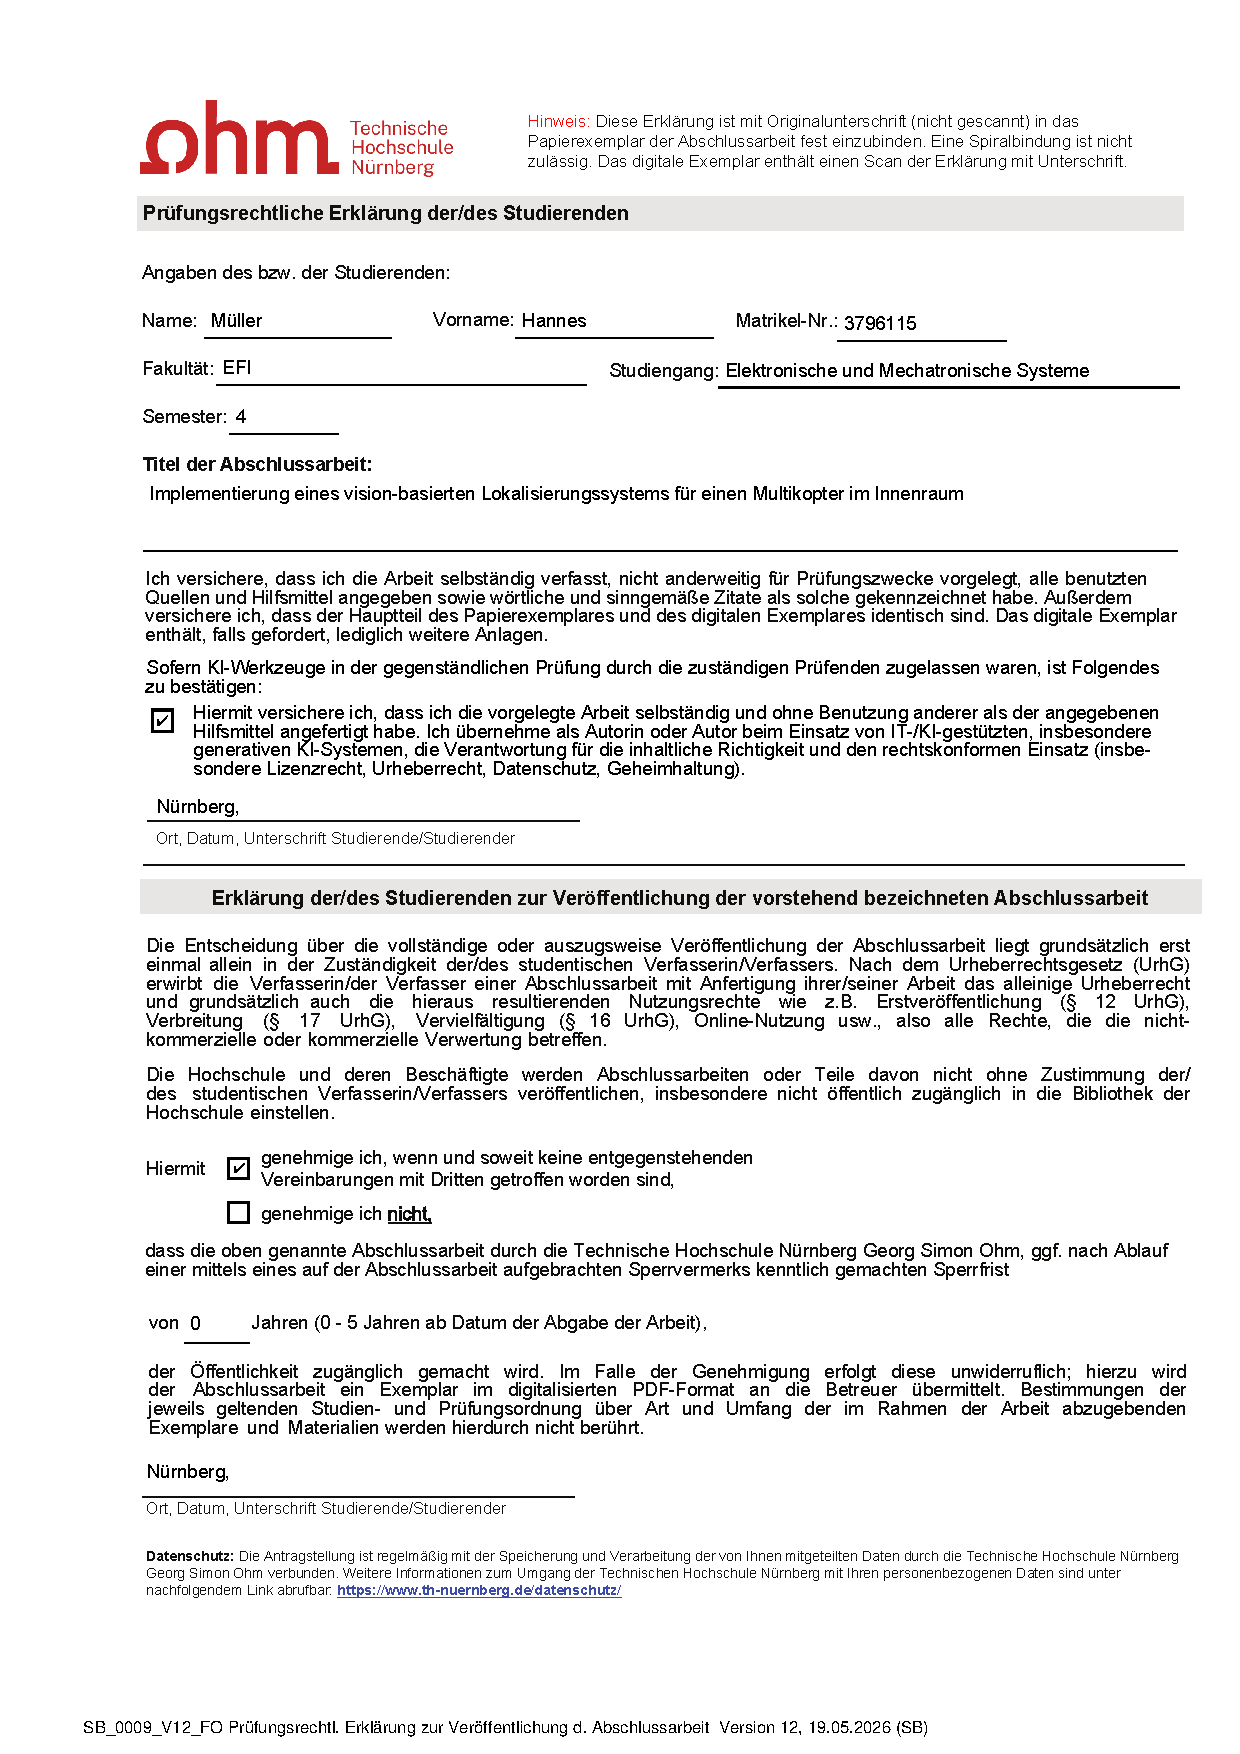
\includepdf[scale=1.0,page=1]{Erklaerung_Hannes.pdf}
  \thispagestyle{empty}
\end{center}

%%%%%%%%%%%%%%%%%%%%%%%%%%%%%%%%%%%%%%%%%%%%%%%%%%%
%%%              Hier Abstract einfügen          %%%
%%%%%%%%%%%%%%%%%%%%%%%%%%%%%%%%%%%%%%%%%%%%%%%%%%%

% Abstract einbinden
%!TeX root=00_Abschlussarbeit.tex

\selectlanguage{english}
\renewcommand{\abstractname}{Abstract}
%\begin{abstract}


\chapter*{Abstract - Noch nicht überarbeitet, Erste Fassung}
\addcontentsline{toc}{chapter}{Abstract}
\noindent
% TEXT ENGLISCH %
This thesis describes the development of a visual localization system for unmanned aerial vehicles based on fiducial markers in indoor environments.
The Robot Operating System 2 is used as the middleware framework; AprilTags are used as the marker framework.
The system uses the RGB images from two cameras as its input data source—one facing forward and one facing downward.
The image processing and navigation calculations are performed by a mini-computer mounted on the aircraft.
Position determination is based on the mapping of fiducial markers using simultaneous localization and mapping.
For the extrinsic calibration of the cameras, a custom-developed algorithm for determining the respective transformation matrix is described.
Position determination itself is achieved by detecting the previously mapped markers and calculating the poses of the camera lenses.
The position data from both sensors are processed, fused into a single pose, and transmitted to the flight controller.
The overall system enables GPS-independent positioning designed for indoor use.
Finally, a prototype application is presented that can be used to control the aircraft.

%\end{abstract}


\selectlanguage{ngerman}
\renewcommand{\abstractname}{Kurzfassung}
%\begin{abstract}
\chapter*{Kurzfassung - Noch nicht überarbeitet, Erste Fassung}
\addcontentsline{toc}{chapter}{Kurzfassung}
\noindent
% TEXT DEUTSCH %
Diese Arbeit beschreibt die Entwicklung eines visuellen Lokalisierungssystems für unbemannte Luftfahrzeuge auf Basis von Fiducial-Markern im Innenraum.
Als Middleware-Framework wird das Robot Operating System 2 verwendet; als Marker-Framework kommen AprilTags zum Einsatz.
Das System nutzt die RGB-Bilder zweier Kameras als Eingangsdatenquelle – eine frontal und eine nach unten ausgerichtet.
Die Berechnungen zur Bildverarbeitung sowie zur Navigation werden durch einen am Luftfahrzeug montierten mini-Computer durchgeführt.
Grundlage der Positionsbestimmung bildet die Kartierung der Fiducial-Marker mittels Simultaner Lokalisierung und Kartierung.
Zur extrinsischen Kalibrierung der Kameras wird ein eigens entwickelter Algorithmus zur Bestimmung der jeweiligen Transformationsmatrix beschrieben.
Die Positionsbestimmung selbst erfolgt durch die Erkennung der zuvor kartierten Marker sowie die Berechnung der Posen der Kameraoptiken.
Die Positionsdaten beider Sensoren werden aufbereitet, zu einer einzigen Pose fusioniert und an den Flugcontroller übermittelt.
Das Gesamtsystem ermöglicht eine GPS-unabhängige Lokalisierung, die für den Einsatz in Innenräumen ausgelegt ist.
Abschließend wird eine prototypische Anwendung vorgestellt, die zur Steuerung des Luftfahrzeugs eingesetzt werden kann.


%\end{abstract}

\selectlanguage{ngerman}
\newpage

% Inhaltsverzeichnis
\pagestyle{plain}

\begingroup
\RedeclareSectionCommand[
  afterskip=0.4\baselineskip
]{chapter}

\tableofcontents
\endgroup

\clearpage

% Abkürzungsverzeichnis
%!TeX root=00_Abschlussarbeit.tex

%chapter*{Abkürzungsverzeichnis}

% \label{sec:abkuerzungsverzeichnis}
\newacronym{uav}{UAV}{Unmanned Aerial Vehicle}
\newacronym{lipo}{LiPo}{Lithium-Polymer-Akku}
\newacronym{imu}{IMU}{Inertial Measurement Unit}
\newacronym{gps}{GPS}{Global Positioning System}

\begingroup
\RedeclareSectionCommand[
  afterskip=0.4\baselineskip
]{chapter}

\printglossary[
  type=acronym,
  style=acronymstyle,
  title=Abkürzungsverzeichnis,
  nogroupskip,
  nonumberlist
]
\endgroup

\clearpage



% Symbolverzeichnis
%!TeX root=00_Abschlussarbeit.tex

%chapter*{Symbolverzeichnis}

% \glsadd{sym:tp} 


\newglossaryentry{sym:xc}{
  type=symbols,
  name={$X_c$},
  description={X-Koordinate des Kamera-Koordinatensystems}
}

\newglossaryentry{sym:yc}{
  type=symbols,
  name={$Y_c$},
  description={Y-Koordinate des Kamera-Koordinatensystems}
}

\newglossaryentry{sym:zc}{
  type=symbols,
  name={$Z_c$},
  description={Z-Koordinate des Kamera-Koordinatensystems}
}

\newglossaryentry{sym:nullc}{
  type=symbols,
  name={$0_c$},
  description={Ursprung des Kamera-Koordinatensystems}
}

\newglossaryentry{sym:xt}{
  type=symbols,
  name={$X_t$},
  description={X-Koordinate des Werkzeug-Koordinatensystems}
}

\newglossaryentry{sym:yt}{
  type=symbols,
  name={$Y_t$},
  description={Y-Koordinate des Werkzeug-Koordinatensystems}
}

\newglossaryentry{sym:zt}{
  type=symbols,
  name={$Z_t$},
  description={Z-Koordinate des Werkzeug-Koordinatensystems}
}

\newglossaryentry{sym:nullt}{
  type=symbols,
  name={$0_t$},
  description={Ursprung des Werkzeug-Koordinatensystems}
}


\newglossaryentry{sym:x1}{
  type=symbols,
  name={$X_1$},
  description={X-Koordinate des Basis-Koordinatensystems}
}

\newglossaryentry{sym:y1}{
  type=symbols,
  name={$Y_1$},
  description={Y-Koordinate des Basis-Koordinatensystems}
}

\newglossaryentry{sym:z1}{
  type=symbols,
  name={$Z_1$},
  description={Z-Koordinate des Basis-Koordinatensystems}
}

\newglossaryentry{sym:null1}{
  type=symbols,
  name={$0_1$},
  description={Ursprung des Basis-Koordinatensystems}
}

\newglossaryentry{sym:A}{
  type=symbols,
  name={$A$},
  description={Saugerfläche}
}

\newglossaryentry{sym:a}{
  type=symbols,
  name={$a$},
  description={Beschleunigung der Handhabungseinrichtung}
}

\newglossaryentry{sym:g}{
  type=symbols,
  name={$g$},
  description={Erdbeschleunigung}
}

\newglossaryentry{sym:m}{
  type=symbols,
  name={$m$},
  description={Masse eines Objekts}
}

\newglossaryentry{sym:F}{
  type=symbols,
  name={$F$},
  description={Festhaltekraft}
}

\newglossaryentry{sym:S}{
  type=symbols,
  name={$S$},
  description={Sicherheitsfaktor bei Vakuumgreifern}
}

\newglossaryentry{sym:p}{
  type=symbols,
  name={$p$},
  description={Vakuum in Prozent}
}

\newglossaryentry{sym:xs}{
  type=symbols,
  name={$x_s$},
  description={Greifbereich}
}

\newglossaryentry{sym:pA}{
  type=symbols,
  name={$p_A$},
  description={Arbeitsdruck}
}

\newglossaryentry{sym:pG}{
  type=symbols,
  name={$p_G$},
  description={Gegendruck}
}

\newglossaryentry{sym:ps}{
  type=symbols,
  name={$p_S$},
  description={Speisedruck}
}

\newglossaryentry{sym:FG}{
  type=symbols,
  name={$F_G$},
  description={Greifkraft}
}

\begingroup
\RedeclareSectionCommand[
  afterskip=0.4\baselineskip
]{chapter}

\printglossary[
  type=symbols,
  style=symstyle,
  title=Symbolverzeichnis,
  nogroupskip,
  nonumberlist
]
\endgroup

\pagestyle{plain}
\newpage
\pagenumbering{arabic}

%%%%%%%%%%%%%%%%%%%%%%%%%%%%%%%%%%%%%%%%%%%%%%%%%%%
%%%                    Text                     %%%
%%%%%%%%%%%%%%%%%%%%%%%%%%%%%%%%%%%%%%%%%%%%%%%%%%%

% Inhaltsdateien einbinden

\chapter{Einleitung}

Unbemannte Fluggeräte werden zunehmend in zivilen Anwendungsbereichen eingesetzt.
Eine grundlegende Voraussetzung für ihren sicheren Betrieb ist die zuverlässige Kenntnis der eigenen Position.
Insbesondere bei einer autonomen Flugführung muss ein Fluggerät seine Lage im Raum fortlaufend bestimmen, um Kollisionen mit Hindernissen zu vermeiden und einen sicheren Flug zu gewährleisten.

Im Außenbereich wird die dafür benötigte Positionsreferenz in der Regel durch Satellitennavigation bereitgestellt.
In Innenräumen steht diese jedoch meist nicht zur Verfügung, da der Satellitenempfang durch die Gebäudestruktur eingeschränkt ist.
Ohne eine externe Positionsreferenz lässt sich die Position nur kurzzeitig aus den im Fluggerät verbauten Sensoren schätzen.
Dabei summieren sich Fehler mit der Zeit auf und führen im Innenraum zwangsläufig zu einer Kollision mit einem Hindernis.
Für einen zuverlässigen Flug im Innenraum ist daher eine alternative Positionsreferenz zwingend erforderlich.

Das Ziel dieser Arbeit ist es, ein unbemanntes Fluggerät zu entwickeln, das sich ohne Satellitennavigation im Innenraum selbst lokalisiert und positioniert.
Die extern berechnete Positionsschätzung soll dem Flugcontroller als Referenz für die Flugsteuerung bereitgestellt werden.
Darüber hinaus ist ein Verfahren zu entwickeln, das eine unbekannte Umgebung vollständig erfasst oder eine bestehende Karte ergänzt und deren Ergebnis der Positionsbestimmung zuführt.


Als Grundgerüst dient ein Multikopter des Typs Holybro X650 mit einem Flugcontroller Pixhawk 6X und einem als Begleitrechner eingesetzten NVIDIA Jetson Orin Nano.
Das Fluggerät ist mit zwei Logitech-Kameras ausgestattet, von denen eine nach unten und eine nach vorne gerichtet ist.
Die entwickelte Lösung ist vollständig aus quelloffener Software und gängigen Komponenten aufgebaut.

Als Grundlage der Positionsreferenz dienen Fiducial-Marker, die in der Flugumgebung angebracht sind.
Unter den betrachteten Fiducial-Marker-Systemen fiel die Wahl auf AprilTags des Typs \texttt{tag36h11}, da diese sich mit der eingesetzten Kartierungsmethode kombinieren lassen und hardwarebeschleunigt erkannt werden können.
Die Lage der Fiducial-Marker zueinander wird in einer vorab erstellten Karte hinterlegt.
Die Auswahl des Kartierungsverfahrens erfolgt über eine Nutzwertanalyse der betrachteten Verfahren zur simultanen Lokalisierung und Kartierung.


Während des Flugs berechnet ein auf dem Fluggerät befestigter Begleitrechner aus den Fiducial-Marker-Detektionen einer nach unten gerichteten Kamera fortlaufend die Pose des Fluggeräts relativ zur Karte.
Die einzelnen Schätzungen werden über eine Ausreißerfilterung bereinigt, anhand der Fiducial-Markergröße, des Abstands und der Güte der Karte gewichtet fusioniert und zeitlich geglättet.
Die so bestimmte Pose wird über eine Kommunikationsschnittstelle an den Flugcontroller übergeben.
Dort wird sie in einem zeitdiskreten Zustandsschätzer mit den übrigen Sensordaten fusioniert und als externe Positionsreferenz verwendet, während Satellitennavigation und Magnetometer von der Fusion ausgeschlossen sind.

Die Arbeit ordnet zunächst bestehende Verfahren zur Lokalisierung ohne Satellitennavigation in den Stand der Technik ein und leitet daraus die gewählte Marker- und Kartierungsmethodik ab.
Darauf folgen die Beschreibung des Gesamtsystems, die Umsetzung der Kartierung und die im Flug ablaufende Positionsbestimmung.
Den Abschluss bilden die Versuchsdurchführung und die Evaluation, in der die erzeugten Karten gegen eine bekannte Referenz verglichen und das Verhalten der Positionsbestimmung in praktischen Flugversuchen bewertet werden.
%!TeX root=00_Abschlussarbeit.tex


% Kapitel des Hauptteils einbinden
%!TeX root=20_Hauptteil.tex

\chapter{Theoretische Grundlagen}

ZZum besseren Verständnis der vorliegenden Arbeit werden im folgenden Kapitel die theoretischen Grundlagen erläutert.
Es werden grundlegende Begriffe aus den Bereichen der Robotik, der Sensorik sowie der visuellen Navigation eingeführt.
Darüber hinaus wird gesondert auf den verwendeten Flugcontroller, die zugrundeliegenden Koordinatensysteme sowie die relevanten Transformationen eingegangen. 


\section{Grundlagen Unbemannter Flugroboter am Beispiel der Holybro X650}
Unter einem unbemannten Luftfahrzeug \gls{uav}, umgangssprachlich auch als Drohne bezeichnet, versteht man ein Fluggerät, welches ohne einen menschlichen Piloten an Bord betrieben werden kann.
Dabei können \gls{uav}s entweder ferngesteuert von einem menschlichen Operator oder vollständig autonom durch einen bordeigenen Computer geführt werden.
Die Anfänge unbemannter Luftfahrzeuge reichen bis in die 1910er Jahre zurück, wo sie vorrangig für militärische Zwecke eingesetzt wurden.
Ab den 2000er Jahren fanden \gls{uav}s zunehmend Eingang in zivile Anwendungsgebiete, wie beispielsweise die Katastrophenhilfe. \cite[S. 1--3]{Studiawan2026}

\subsection{Aufbau der Holybro X650}
\textbf{Grundrahmen} Der Grundrahmen eines UAV dient als mechanische Basis für die Montage aller weiteren Komponenten.
Das Design des Rahmens beeinflusst maßgeblich die Flugeigenschaften des Geräts.
Das in dieser Arbeit verwendete Modell ist als Senkrechtstarter konzipiert und basiert auf einem X-förmigen Quadcopter-Rahmen.
Die wesentlichen Bestandteile des Rahmens umfassen die Ausleger, das Landegestell sowie die zentrale Montageplattform für die Elektronik.
Die Holybro X650 weist eine Diagonale von 650 mm auf.
Abbildung \ref{fig:roll_pitch_yaw} zeigt ein Bild der Holybro X650.
 \cite{Wu2021} \cite{holybro_x650}

\noindent
\textbf{Antriebssystem} Das Antriebssystem besteht aus vier Elektromotoren, die jeweils an einem der Ausleger montiert sind.
An den Motoren sind Propeller befestigt, welche den erforderlichen Auftrieb erzeugen.

\noindent
\textbf{Flugcontroller} Der Flugcontroller bildet das zentrale Steuerungselement eines UAV.
Er setzt eingehende Steuerbefehle in konkrete Ansteuersignale um, die an die Motoren weitergeleitet werden.
In Kapitel \ref{sec:PX4 Autopilot} wird näher auf den verwendeten Flugcontroller eingegangen.

\noindent
\textbf{Energieversorgung} Die Energieversorgung erfolgt über einen \gls{lipo} mit einer Nennspannung von 14,8 V.
Das verbaute Power Module wandelt diese Spannung auf 5,2 V, mit welcher sowohl die Steuerelektronik als auch die Motoren versorgt werden.

\noindent
\textbf{Nutzlast} Das maximale Abfluggewicht der Holybro X650 beträgt 6,3 kg, wobei der flugfertige Grundrahmen bereits ein Eigengewicht von 4,3 kg aufweist.
Daraus ergibt sich eine maximale Nutzlast von 2 kg (ohne Akku). \cite{holybro_x650}

\section{Koordinatensysteme und Transformationen}
Dieses Kapitel behandelt die verschiedenen Koordinatensysteme, die in dieser Arbeit relevant sind.
Dabei wird zwischen dem Welt-, Roboter-, Kamera- und Fiducialkoordinatensystem unterschieden.
Weiterhin werden die grundlegenden Konzepte zur Repräsentation von Position und Orientierung im Raum erläutert.
Abschließend wird auf die notwendigen Koordinatentransformationen eingegangen.

\subsection{Vergleich von Welt-, Roboter-, Kamera- und Fiducialkoordinatensystem}
Ein Koordinatensystem ist ein mathematisches Konstrukt, das zur eindeutigen Beschreibung der Lage von Punkten im Raum verwendet wird.
Zur Beschreibung von Bewegungen ist die Festlegung eines Koordinatensystems von entscheidender Bedeutung.
Es besteht aus einem Bezugspunkt, dem Ursprung, sowie drei orthogonalen Achsen, die als X-, Y- und Z-Achse bezeichnet werden.
In dieser Arbeit wird standardmäßig das rechtshändige Koordinatensystem verwendet. \cite[S. 17]{ISO8855}
Mathematisch wird der Zusammenhang durch
\begin{equation}
\mathbf{Z} = \mathbf{X} \times \mathbf{Y}
\label{eq:rechte_hand_regel}
\end{equation}
dargestellt.
In dieser Arbeit werden die Achsen entsprechend des informellen Industriestandards wie folgt dargestellt: X-Achse in Rot, Y-Achse in Grün und Z-Achse in Blau.
Ein Überblick über die in dieser Arbeit verwendeten Koordinatensysteme ist in Abbildung \ref{fig:Koordinatensysteme} dargestellt.

\begin{figure}[htbp]
\centering
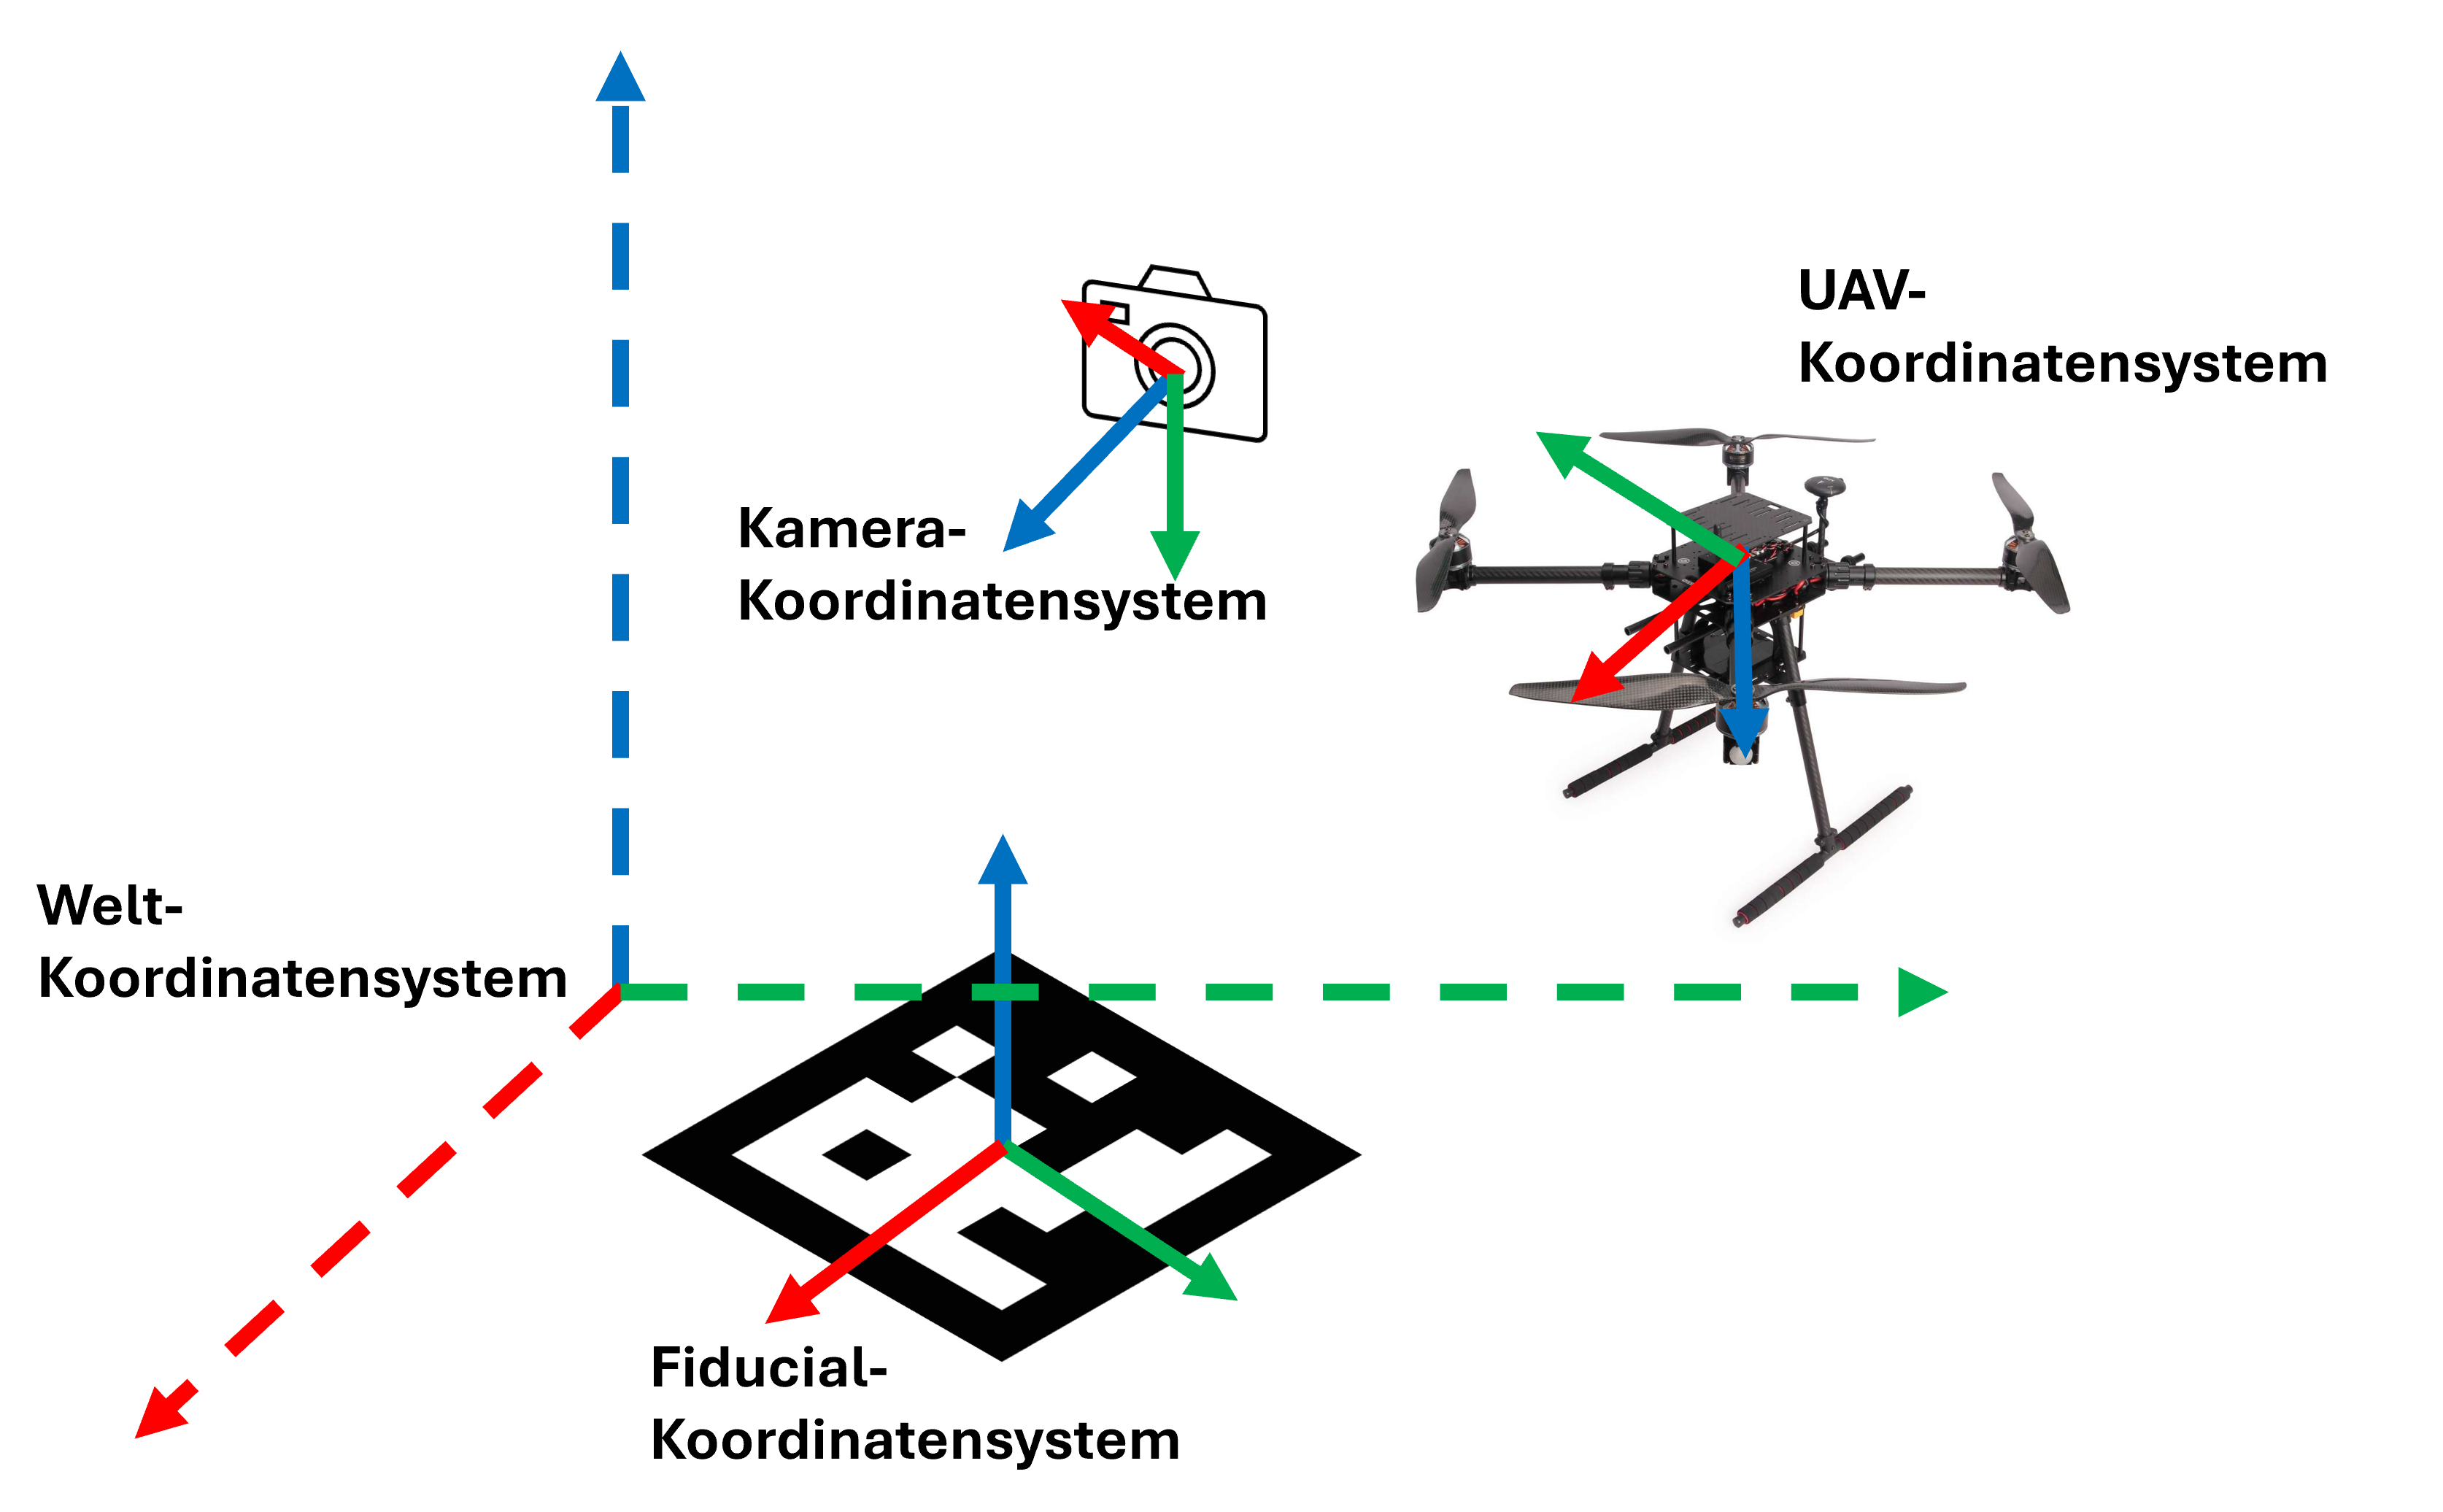
\includegraphics[width=1.0\textwidth]{Bilder/Koordinatensysteme.png}
\caption{Vergleich der Koordinatensysteme \cite{holybro_x650}}
\label{fig:Koordinatensysteme}
\end{figure}
\FloatBarrier

Das Weltkoordinatensystem dient als globaler Referenzrahmen, in dem die Position aller Objekte beschrieben wird.
Der Ursprung dieses Koordinatensystems kann frei gewählt werden und wird durch die Variable $O_0$ repräsentiert.
Die Achsen werden durch $X_0$, $Y_0$ und $Z_0$ dargestellt \cite[S. 4]{ISO9787}.

Das UAV-Koordinatensystem ist in der Regel vom Hersteller vorgegeben und richtet sich in diesem konkreten Fall nach dem Flugregler.
In der zugehörigen Dokumentation wird angegeben, dass die X-Achse ($X_u$) nach vorne, die Y-Achse ($Y_u$) 
nach rechts und die Z-Achse ($Z_u$) nach unten zeigt.
Der Ursprung dieses Koordinatensystems ($O_u$) befindet sich im Zentrum des Flugreglers \cite{PX4Frames}.

Das Kamerakoordinatensystem ist in der Regel so definiert, dass die Z-Achse ($Z_c$) entlang der optischen Achse der Kamera zeigt, 
die X-Achse ($X_c$) nach rechts auf der Bildebene und die Y-Achse ($Y_c$) nach unten auf der Bildebene zeigt.
Der Ursprung ($O_c$) befindet sich im optischen Zentrum der Kamera. \cite[S. 44]{Szeliski2022}

Das Fiducialkoordinatensystem ist in dieser Arbeit so definiert, dass sich der Ursprung ($O_f$) im Mittelpunkt der Fiducialmarke befindet.
Die Z-Achse ($Z_f$) zeigt senkrecht aus der Markerebene heraus, die X-Achse ($X_f$) zeigt nach rechts in der Markerebene und die Y-Achse ($Y_f$) 
zeigt nach oben in der Markerebene.



\subsection{Repräsentation von Position und Orientierung}
In diesem unterkapitel wird das verwendetet \gls{uav} als starrer Körper betrachtet. 
Die vollständige Beschreibung der Lage eines starren Körpers im Raum erfolgt durch seine Position und Orientierung \cite[38]{Siciliano2009}.

Die Position eines Körpers wird durch den Vektor
\begin{equation}
\mathbf{p} = (x, y, z)^T
\label{eq:position_vektor}
\end{equation}
beschrieben. 
Wobei die Koordinaten einen bestimmten Koordinatensystem zugeordnet sind. 

Die Orientierung eines Körpers kann auf verschiedene Weisen dargestellt werden. 
Im Folgenden werden die zum Verständnis dieser Arbeit relevanten Darstellungsformen erläutert.
Grundsätzlich kann sich ein Körper um drei Achsen drehen, was durch die Euler-Winkel Roll ($\phi$), Pitch ($\theta$) und Yaw ($\psi$) beschrieben wird.
Abbildung \ref{fig:roll_pitch_yaw} zeigt die Definition dieser Winkel am Beispiel der Holybro X650.
Die Pfeilrichtung entspricht der positiven Drehrichtung im rechtshändigen Koordinatensystem.
\begin{figure}[htbp]
   \centering
   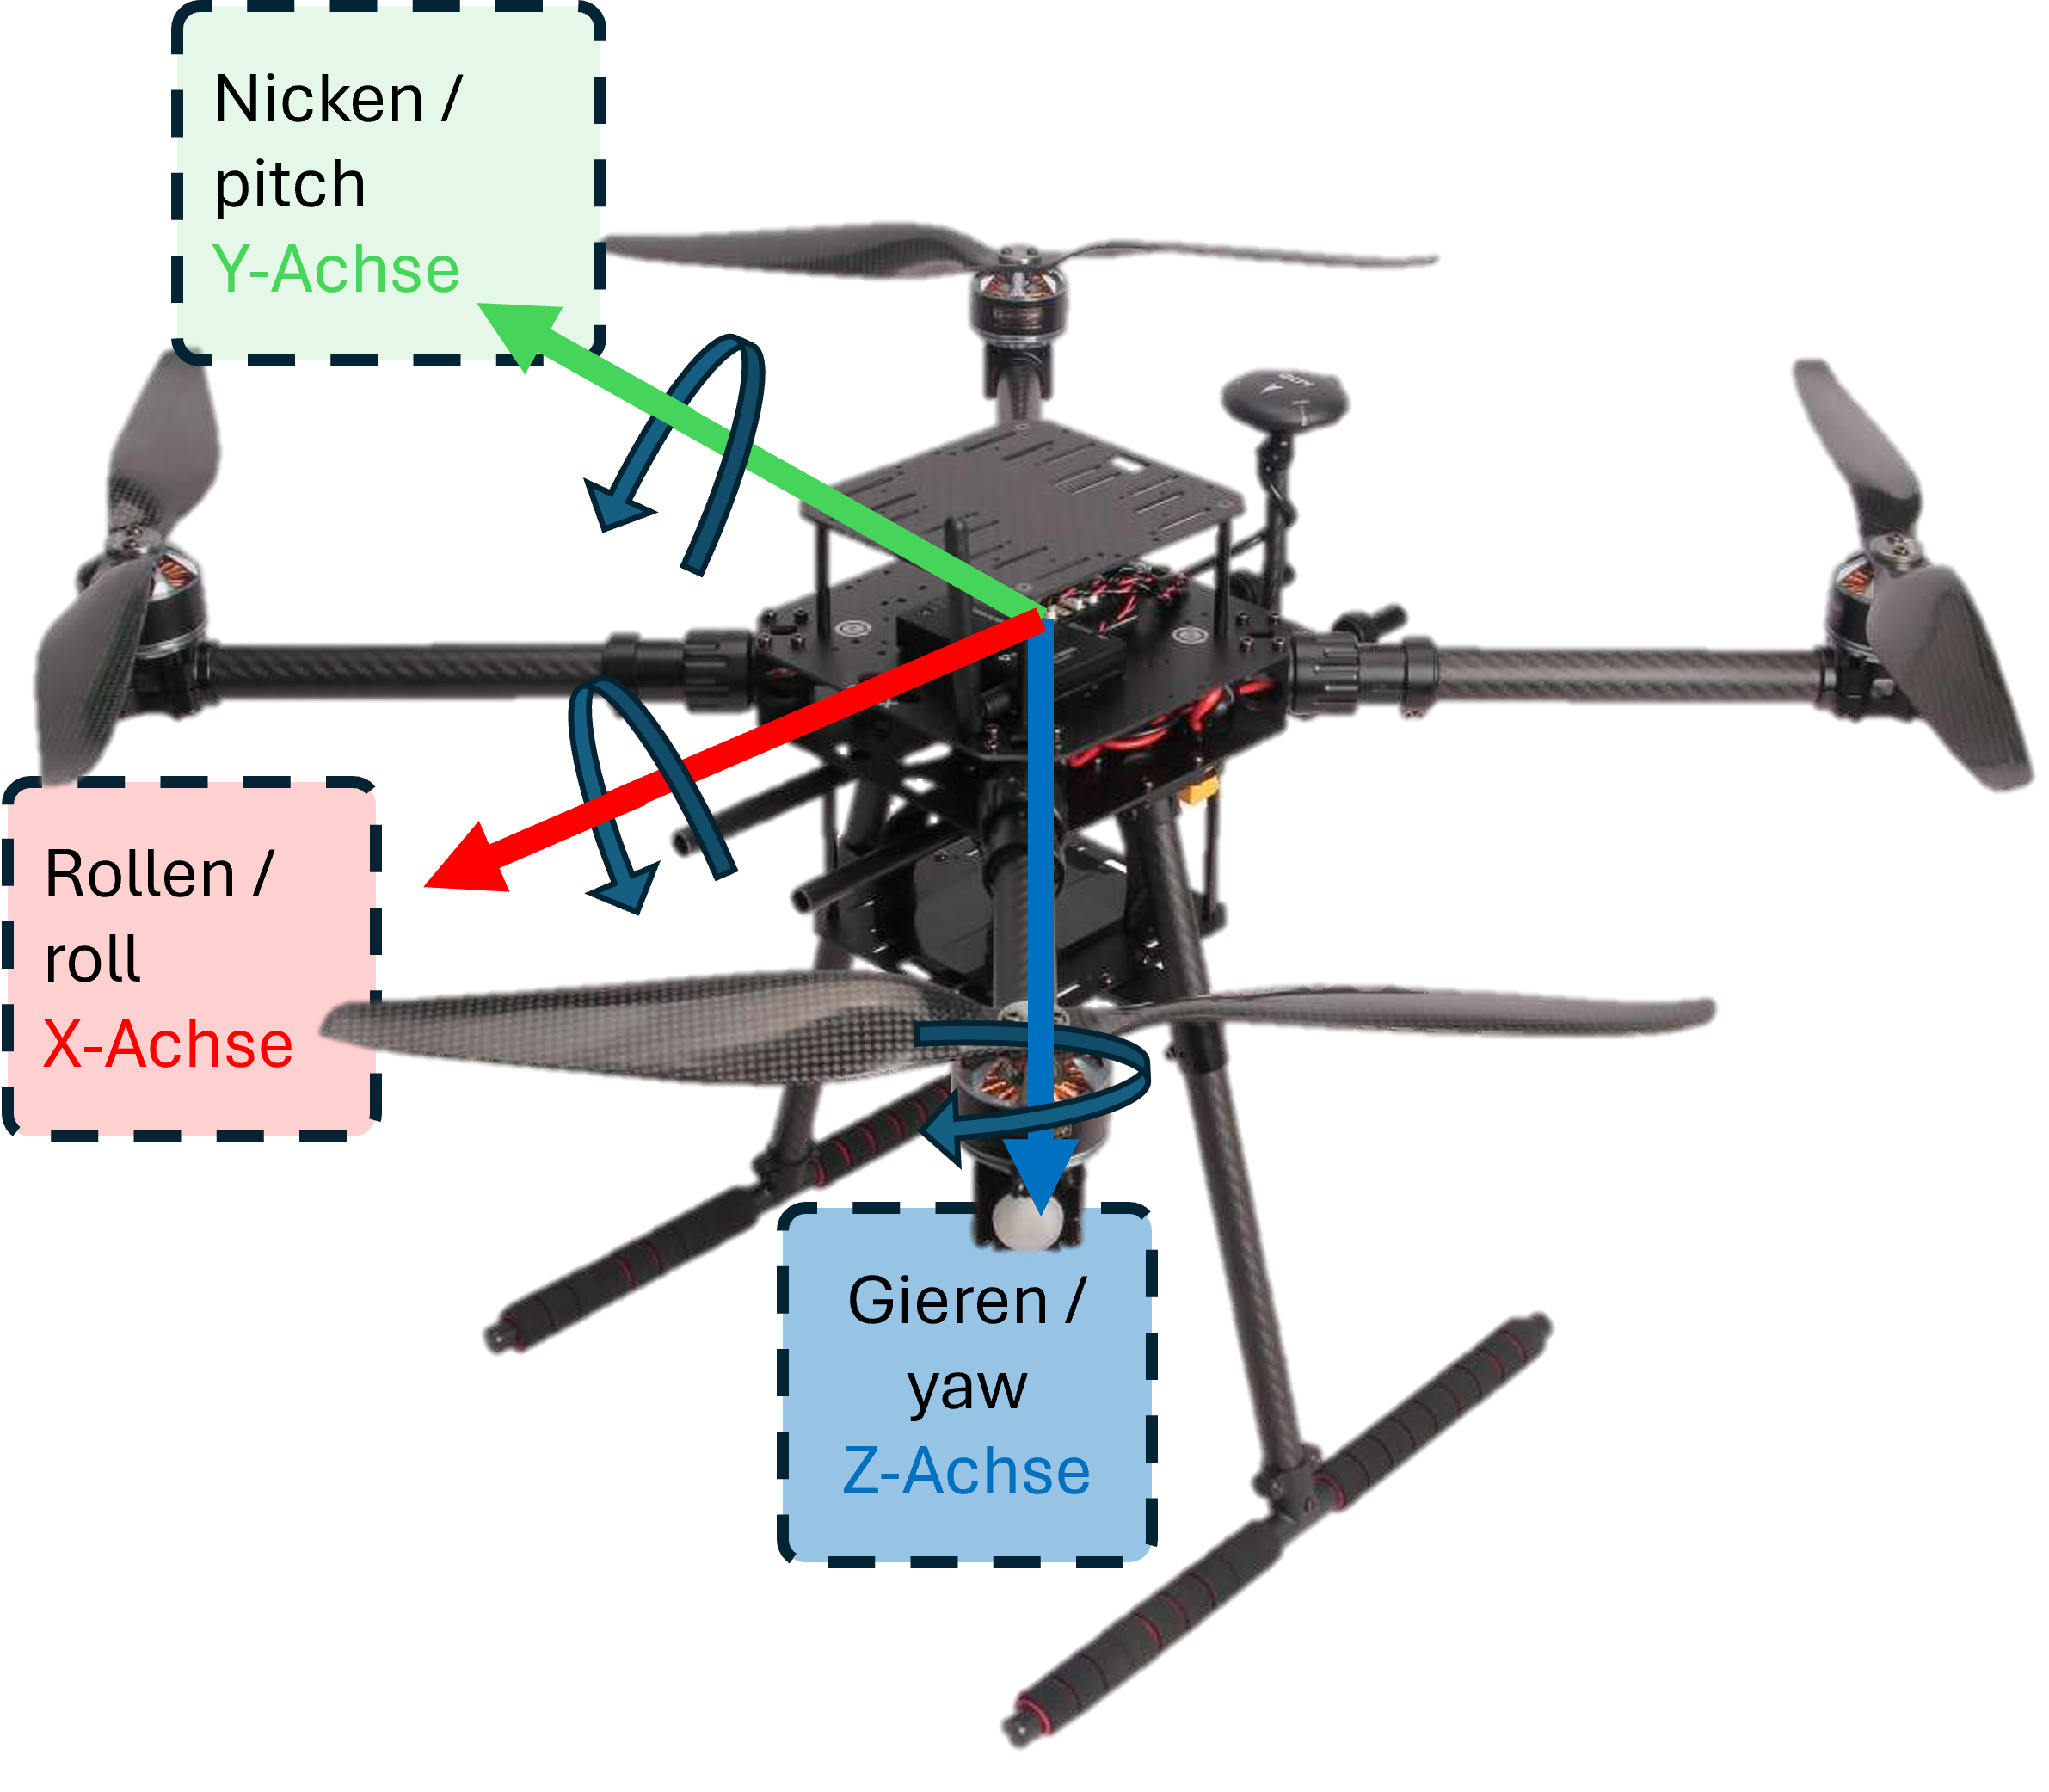
\includegraphics[width=1.0\textwidth]{Bilder/Roll_Yaw_Pitch.png}
   \caption{Roll, Pitch und Yaw am Beispiel Holybro X650 \cite{holybro_x650}}
   \label{fig:roll_pitch_yaw}
\end{figure}
\FloatBarrier

Die folgenden Ausführungen zu Quaternionen beziehen sich auf \cite[15-16]{2016}.
Weiterhin kann die Orientierung als sogenanntes Quaternion dargestellt werden.
Quaternionen bieten gegenüber Euler-Winkeln den Vorteil, dass sie keine Singularitäten (Gimbal Lock) aufweisen.
Quaternionen stellen eine Erweiterung des komplexen Zahlenraums dar und werden durch Gleichung \ref{eq:quaternion} definiert.
\begin{equation}
\mathbf{q} = w + ix + jy + kz
\label{eq:quaternion}
\end{equation}
wobei die Komponenten $w$, $x$, $y$ und $z$ reelle Zahlen sind Skalare sind und $i$, $j$ und $k$ die imaginären Einheiten darstellen.
Die Imaginären Einheiten erfüllen die folgenden Multiplikationsregeln:
\begin{equation}
ii = jj = kk = ijk = -1
\label{eq:quaternion_regeln}
\end{equation}

\begin{equation}
ij = k , \quad jk = i , \quad ki = j
\label{eq:quaternion_regeln2}
\end{equation}

\begin{equation}
ji = -k , \quad kj = -i , \quad ik = -j
\label{eq:quaternion_regeln3}
\end{equation}

Addition und Multiplikation von Quaternionen werden entsprechend den Formeln \ref{eq:quaternion_addition} und \ref{eq:quaternion_multiplikation} definiert.
\begin{equation}
q_1 + q_2 = (w_1 + w_2) + i(x_1 + x_2) + j(y_1 + y_2) + k(z_1 + z_2)
\label{eq:quaternion_addition}
\end{equation}
\begin{equation}
\begin{split}
q_1 \cdot q_2 = &(w_1 w_2 - x_1 x_2 - y_1 y_2 - z_1 z_2) \\
+ &i(w_1 x_2 + x_1 w_2 + y_1 z_2 - z_1 y_2) \\
+ &j(w_1 y_2 - x_1 z_2 + y_1 w_2 + z_1 x_2) \\
+ &k(w_1 z_2 + x_1 y_2 - y_1 x_2 + z_1 w_2)
\end{split}
\label{eq:quaternion_multiplikation}
\end{equation}

Das Einheitsquaternion oder auch Rotationsquaternion $\mathbf{q}$ beschreibt eine Rotation um den Winkel $\phi$ 
um eine normierte Rotationsachse $\mathbf{v} = (v_x, v_y, v_z)^T$ und wird durch Gleichung \ref{eq:einheitsquaternion} beschrieben. 

\begin{equation}
\mathbf{q} = \left(\cos\frac{\phi}{2},\ \mathbf{v} \cdot \sin\frac{\phi}{2}\right) = \left(\cos\frac{\phi}{2},\ v_x \sin\frac{\phi}{2},\ v_y \sin\frac{\phi}{2},\ v_z \sin\frac{\phi}{2}\right)
\label{eq:einheitsquaternion}
\end{equation}

Die Konjunktion eines Quaternions ist analog zu den komplexen Zahlen mit der Gleichung \ref{eq:quaternion_konjungiert} beschrieben. 
\begin{equation}
\bar{\mathbf{q}} = (w, -x, -y, -z)
\label{eq:quaternion_konjugiert}
\end{equation}

Für die Rotation eines beliebigen Punktes $\mathbf{p} = (0, p_x, p_y, p_z)$ um ein 
Rotationsquaternion $\mathbf{q}$ kann nun die Gleichung \ref{eq:quaternion_rotation} angewendet werden. \cite[S. 112]{Quan2017}

\begin{equation}
\mathbf{p}' = \mathbf{q} \cdot \mathbf{p} \cdot \bar{\mathbf{q}}
\label{eq:quaternion_rotation}
\end{equation}

\subsection{Transformation von Koordinatensystemen}

\subsection{Repräsentation von Position}
Ein Punkt in einem Raum wird durch einen Vektor 

\subsection{Repräsentation von Orientierung}

 

\section{Autopilot PX4-6C}
\label{sec:PX4 Autopilot}
Hier einfach schreiben...
\subsection{Architektur}
Hier einfach schreiben...

\subsection{Sensorintegration}
Hier einfach schreiben...

\subsection{Kommunikationsschnittstellen}
Hier einfach schreiben...

\subsection{Echtzeitfähikgkeit}


\subsection{Vergleich von Kamera-, Roboter- und Weltkoordinatensystem}

\subsection{Transformation von Koordinatensystemen}

\section{Visuelle Navigation}

\subsubsection{Sensorik zur visuellen Navigation}

\subsubsection{Grundlagen der Fiduccial-Erkennung}
\subsubsection{PNP-Fehler}

\subsubsection{Visuelle Odometrie}






%!TeX root=20_Hauptteil.tex

\chapter{Stand der Technik}

Dieses Kapitel gibt einen Überblick über den aktuellen Stand der Technik im Bereich 
der \gls{gnss}-freien Lokalisierung von \gls{uav} und ordnet die in dieser Arbeit 
gewählten Methoden in den wissenschaftlichen Kontext ein.
Zunächst werden bestehende Lokalisierungsansätze ohne \gls{gnss} vorgestellt und hinsichtlich ihrer Eignung für Innenraumanwendungen bewertet.
Anschließend werden verschiedene Fiducial-Marker-Systeme verglichen und deren Eigenschaften im Hinblick auf die Anforderungen dieser Arbeit diskutiert.
Abschließend wird auf die simultane Lokalisierung und Kartierung eingegangen, die die Grundlage für die in dieser Arbeit verwendete Kartierungsmethodik bildet.

\section{GNSS-freie Lokalisierung von UAVs}
Die Navigation ohne \gls{gnss} stellt in der Luftfahrt eine erhebliche Herausforderung dar, da \gls{gnss} als primäre Quelle absoluter Positionsinformationen dient.
In dessen Abwesenheit muss die Position aus der Integration fehlerbehafteter Inertialmessungen 
geschätzt werden, was, wie in Abschnitt \ref{sec:Sensorsysteme} beschrieben, zu einem zeitlich anwachsenden Positionsfehler führt.
Daher ist es notwendig, diesen Fehler durch absolute oder relative Lokalisierungsmethoden auszugleichen.\cite{Jarraya2025}


\subsection{Absolute Lokalisierung}
Absolute Lokalisierungsverfahren spielen eine wichtige Rolle, wenn die genaue Position eines \gls{uav} bezogen auf einen globalen Referenzrahmen bekannt sein muss.\cite{Jarraya2025}
Die gängigste Methode zur Umsetzung einer absoluten Lokalisierung ist ein satellitengestütztes System wie \gls{gps} oder Galileo.
Da in der für diese Arbeit relevanten Flugumgebung kein ausreichender Satellitenempfang herrscht, finden diese Systeme keine Anwendung.
Eine weitere Möglichkeit der absoluten Lokalisierung bieten Template- und Feature-basierte Verfahren sowie Semantic Mapping.

Bei Template- beziehungsweise Feature-basierten Verfahren werden Aufnahmen des \gls{uav} mit bekannten Referenzbildern oder gespeicherten Merkmalen verglichen.
Diese Systeme berücksichtigen ausschließlich visuelle Merkmale, ohne semantische Beziehungen einzubeziehen.\cite{Jarraya2025}
Ein verwandtes Konzept stellen Fiducial-Marker dar, bei denen anstelle natürlicher Bildmerkmale künstlich erzeugte, eindeutig kodierte Muster als Referenz dienen.
Durch ihre definierte Geometrie und Kodierung ermöglichen sie eine präzisere und robustere Posenschätzung als natürliche Bildmerkmale, weshalb sie in dieser Arbeit 
als Grundlage der Lokalisierung eingesetzt werden.
Im Sinne einer globalen absoluten Lokalisierung im Weltkoordinatensystem sind Template- und Feature-basierte Verfahren für Innenraumanwendungen jedoch wenig geeignet, 
da geeignete Referenzdaten schwer zu erfassen sind.\cite{Jarraya2025}

Semantic Mapping verfolgt einen ähnlichen Ansatz: Auch hier werden zunächst Referenzdaten 
erstellt, die anschließend mit aktuell erfassten Daten abgeglichen werden.
Der Unterschied liegt darin, dass nicht nur visuelle Merkmale, sondern auch semantische 
Beziehungen berücksichtigt werden, so wird beispielsweise ein Tisch als Tisch und eine 
Treppe als Treppe interpretiert.\cite{Jarraya2025}
Dieses Verfahren findet in der vorliegenden Arbeit keine Anwendung, da die Erkennungsleistung stark von der Stabilität der jeweiligen Umgebung abhängig ist.

Da die einzige praktikabel umsetzbare Methode der absoluten Lokalisierung ein 
satellitengestütztes System darstellt, welches wie bereits erwähnt in der vorliegenden Umgebung nicht verfügbar ist, wird in dieser Arbeit auf absolute Lokalisierungsverfahren verzichtet 
und ausschließlich relative Lokalisierungsmethoden betrachtet.
Die grundlegende Methodik der zuvor vorgestellten Verfahren findet dabei ebenfalls Anwendung, jedoch ohne Bezug zu einem globalen Referenzrahmen.

\subsection{Relative Lokalisierung}
\label{sec:relative_lokalisierung}
Die relative Lokalisierung zielt darauf ab, die Position und Orientierung eines \gls{uav} innerhalb eines lokalen Koordinatensystems zu bestimmen.
Die Position wird dabei bezogen auf einen definierten Referenzpunkt ermittelt.
Im Folgenden werden die gängigsten Methoden vorgestellt und hinsichtlich ihrer Eignung für die vorliegende Innenraumanwendung bewertet.

\subsubsection{Dead Reckoning Localization}
Bei der \gls{drl} handelt es sich um ein Verfahren, bei dem die aktuelle Position eines 
Objekts ausgehend von einem letzten bekannten Startpunkt kontinuierlich berechnet 
wird.\cite{9982087}
Die Berechnung erfolgt auf Basis der bereitgestellten \gls{imu}-Daten durch Integration 
dieser.
Wie in Abschnitt \ref{sec:sensorik} bereits beschrieben, wirken auf die Sensoren erhebliche 
Fehler, sodass die direkte Integration der rohen \gls{imu}-Messdaten zu großen 
Translationsfehlern führt.
Aus diesem Grund ist eine Filterung der Eingangsdaten notwendig.
Am weitesten verbreitet sind hierbei verschiedene Abwandlungen des Kalman-Filters.

Experimentelle Untersuchungen mit dem \gls{px4}-Autopiloten und einem handelsüblichen 
Pixhawk-Flugregler zeigen, dass der \gls{ekf2} bereits nach 7 Sekunden eine 
Geschwindigkeitsabweichung von $\sigma_{\text{vel}} \approx 0{,}024$~m/s aufweist, was zu 
einem zunehmenden Positionsfehler im Dezimeterbereich führt.\cite{9172736}
Verschiedene Arbeiten zeigen, dass sich der Drift vor allem durch Nutzung verbesserter 
Algorithmen wie dem \gls{iekf} minimieren, jedoch nicht vollständig vermeiden lässt.
\cite{9982087}\cite{9172736}\cite{Ko2018}
Da im verwendeten Flugcontroller, wie in Kapitel \ref{sec:Pixhawk_6X} beschrieben, der 
\gls{ekf} implementiert ist, wird nicht weiter auf andere Abwandlungen des Algorithmus 
eingegangen.

Grundsätzlich ist \gls{drl} für den Innenraum nur zeitlich begrenzt geeignet und als 
primäre Positionsquelle nicht ausreichend.
Im Normalfall wird \gls{drl} daher als Fallback-Strategie genutzt, wenn die primäre 
Positionsquelle nicht verfügbar ist.\cite{9172736}
In dieser Arbeit wird der Flugcontroller entsprechend konfiguriert.


\subsubsection{Visuelle Odometrie und optischer Fluss}
Visuelle Odometrie sowie optischer Fluss sind grundlegende Verfahren zur Lokalisierung eines \gls{uav}.
Die \gls{vo} schätzt die Bewegung einer Kamera anhand sequenzieller Bilddaten, ohne eine Karte der Umgebung zu erstellen.
Dabei werden markante Bildpunkte, auch Landmarken genannt, zwischen aufeinanderfolgenden Frames verfolgt und aus deren Verschiebung auf die Kamerabewegung geschlossen.\cite{Jarraya2025}

Darüber hinaus existieren \gls{vio}-Ansätze, die die Robustheit der \gls{vo} durch Einbeziehen von \gls{imu}-Informationen verbessern.\cite{9836067}
Die visuellen Daten können dabei den Drift der \gls{imu} reduzieren, während die \gls{imu}-Daten den metrischen Maßstab sowie Roll- und Nickwinkel aus den visuellen 
Daten wiederherstellen können.\cite{9836067}
Es gibt sowohl mono- als auch stereokamerabasierte Ansätze, wobei Stereokameras aufgrund der direkten Tiefenschätzung eine höhere Genauigkeit erzielen.\cite{9836067}
Die Fusion von \gls{imu} und \gls{vo} zu \gls{vio} erfolgt typischerweise über einen \gls{ekf}.\cite{9836067}

Da \gls{vo} und \gls{vio} keinen absoluten Positionsbezug besitzen, akkumulieren diese Verfahren über die Zeit einen Drift und sind damit nur bedingt für eine langfristig stabile Innenraumlokalisierung geeignet.\cite{Jarraya2025}
Zudem ist die Leistung kamerabasierter Verfahren stark von den Lichtverhältnissen der Umgebung abhängig.\cite{9836067}
Weiterhin visuelle Odometrie setzt strukturierte Umgebungen voraus, welche in der Versuchsumgebung nicht ohne weiteres gegeben sind. 

Der optische Fluss stellt ein verwandtes Verfahren dar, das im Gegensatz zur \gls{vo} 
lediglich zweidimensionale Geschwindigkeitsinformationen liefert.\cite{Jarraya2025}
Aus diesem Grund ist der optische Flow nicht zur Positionserkennung einer \gls{uav} geeignet.


\subsection{Simultane Lokalisierung und Kartierung}
\gls{slam} beschreibt eine Problemstellung an der Schnittstelle von Computer Vision und Robotik.
Dabei geht es um die selbstständige Erstellung einer Karte einer unbekannten Umgebung bei gleichzeitiger Bestimmung der eigenen Position 
innerhalb dieser Umgebung.\cite{10169695}
Der Begriff simultan beschreibt genau diesen Zusammenhang: 
Kartierung und Positionsbestimmung müssen parallel erfolgen, da jede Aufgabe die andere voraussetzt.\cite{10169695}
Die Lösung dieses Problems erfolgt üblicherweise durch filterbasierte Methoden, wie den \gls{ekf}, oder durch optimierungsbasierte Methoden, die im Folgenden 
näher beschrieben werden.\cite{10169695}

Filterbasierte \gls{slam} Algorithmen verarbeiten Messungen sequenziell und lassen keine Korrektur von vergangenen Messungen zu.
Insbesondere fehlt filterbasierten Methoden die Fähigkeit zur globalen Kartenkorrektur durch Loop Closure, 
was zu einer geringeren Kartierungsgenauigkeit im Vergleich zu optimierungsbasierten Methoden führt.
In der Lokalisierung sind filterbasierte Methoden aufgrund ihrer geringeren Rechenkomplexität jedoch schneller.\cite{10169695}
Der aktuelle Standard bei \gls{slam}-Algorithmen sind optimierungsbasierte Methoden.
 

\subsubsection{Phasen optimierungsbasierter SLAM Methoden}
\label{sec:phasen_slam}
Der allgemeine optimierungsbasierte \gls{slam}-Prozess lässt sich in folgende Phasen unterteilen:

\textbf{Feature Extraction} bezeichnet die Extraktion markanter Merkmale 
aus den Sensordaten, die als Grundlage für die spätere Zuordnung dienen.\cite{10169695}

\textbf{Feature Matching} beschreibt den Abgleich extrahierter Merkmale zwischen 
aufeinanderfolgenden Frames, um die Bewegung des Systems zu schätzen.\cite{10169695}
Beispiele dieser Methoden werden in Abschnitt \ref{sec:relative_lokalisierung} beschrieben.

\textbf{Map Initialization} bezeichnet die Initialisierung der Karte zu Beginn des \gls{slam}-Prozesses.
Dabei werden zunächst markante Bildmerkmale aus den ersten Frames extrahiert und 
einander zugeordnet, um die initiale Struktur der Umgebung zu schätzen.
Aus diesen Zuordnungen werden erste Kartenpunkte sowie deren räumliche Positionen im dreidimensionalen Raum bestimmt.
Die Map Initialization bildet die Grundlage, auf der alle weiteren Kartenpunkte und Posenschätzungen aufgebaut werden. \cite{vslam_core_modules_2024}

\textbf{Loop Closure} bezeichnet die Erkennung bereits besuchter Orte.
Wird ein solcher Ort erkannt, wird die akkumuliert Abweichung anhand gespeicherter Merkmale berechnet und als zusätzlicher Constraint den Faktorgraphen eingetragen. 
Die anschließende globale Optimierung verbessert die Konsistenz der gesamten Karte erheblich. \cite{10169695} 
Der schematische Ablauf von Loop Closure ist in Abbildung~\ref{fig:loop_closure} dargestellt.
Die Funktion des Faktorgraph wird in Abschschnitt \ref{sec:Faktorgraph} näher beschrieben.
\begin{figure}[htbp]
    \centering
    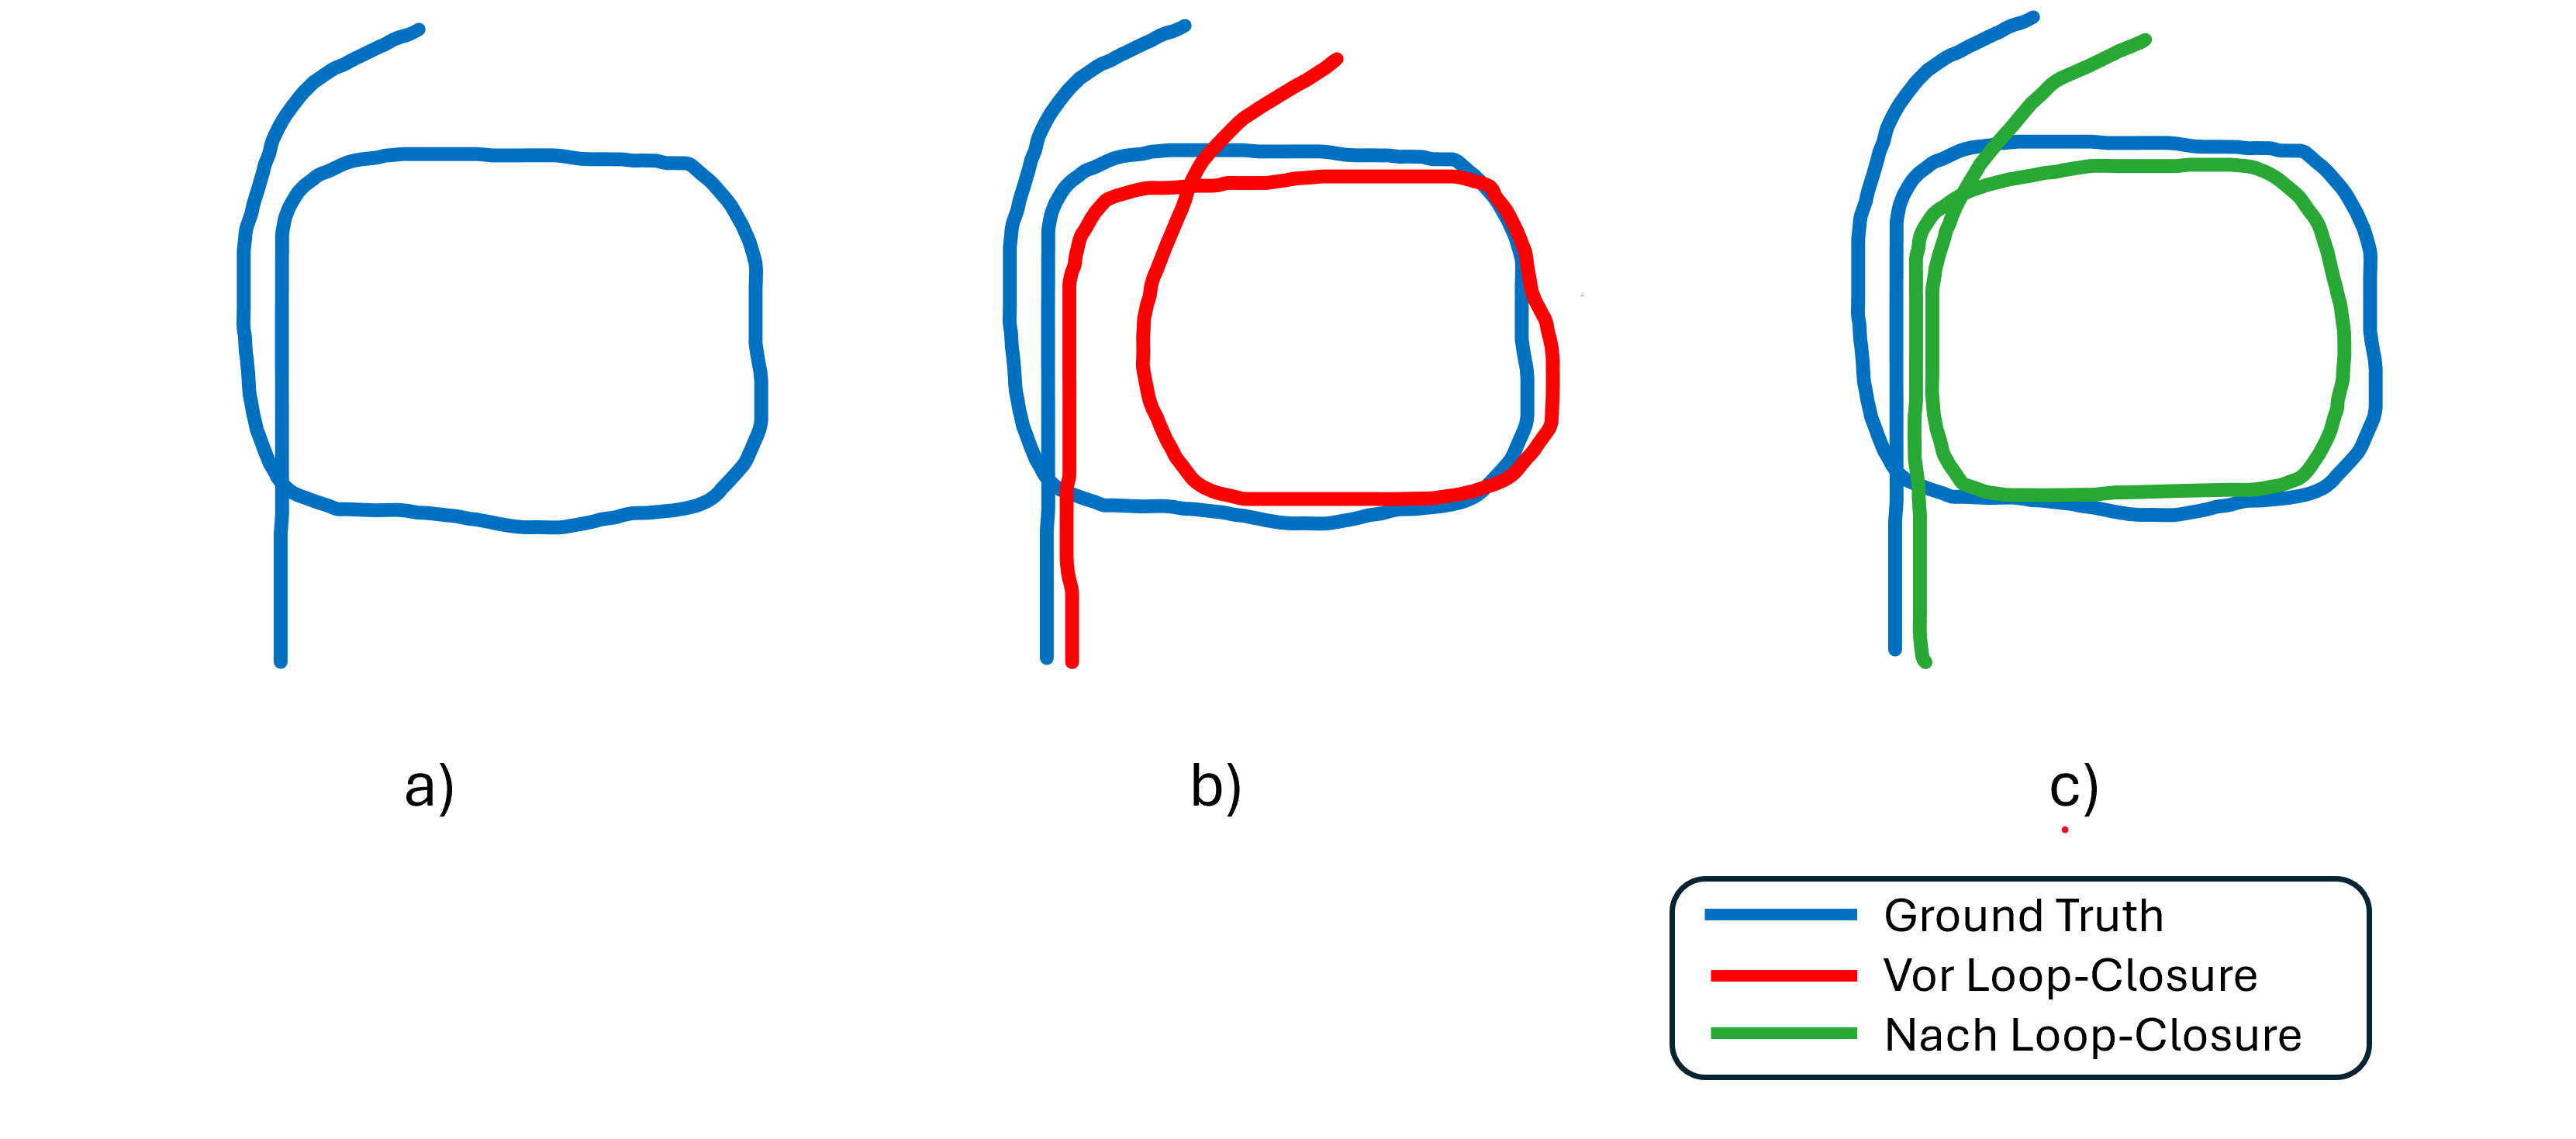
\includegraphics[width=1.0\textwidth]{Bilder/Loop_Closure.png}
    \caption{Veranschaulichung des Loop-Closure-Effekts: 
    (a) Reale Trajektorie ohne akkumulierten Fehler. 
    (b) Geschätzte Trajektorie mit akkumuliertem Drift ohne Loop Closure. 
    (c) Korrigierte Trajektorie nach Anwendung von Loop Closure mit 
    reduziertem akkumuliertem Drift. vgl. \cite{gong_loop_closure}}
    \label{fig:loop_closure}
\end{figure}
\FloatBarrier




\subsubsection{Faktorgraph}
\label{sec:Faktorgraph}
Im folgenden Abschnitt wird der Faktorgraph nur schematisch erläutert, um ein grundsätzliches Verständnis dieser Methodik zu erlangen.
Genaue Herleitungen sowie die Mathematik hinter dem Prinzip können den Quellen \cite{Lai2022}, \cite{Dellaert2017} und \cite{Cai2024} entnommen werden.

Ein Faktorgraph ist eine grafische Darstellung eines Schätzproblems und besteht aus zwei Arten von Knoten: Variablenknoten und Faktorknoten.\cite{Lai2022}
Die Variablenknoten sind die unbekannten Größen, die geschätzt werden sollen -- bei \gls{slam} die Pose des \gls{uav} und die Position der Landmarken.\cite{Lai2022}
Die Faktorknoten verbinden diese Variablen und repräsentieren die Messungen oder das Vorwissen.\cite{Lai2022}

Der Faktorgraph in Abbildung~\ref{fig:Faktorgraph_vereinfacht} zeigt die grundlegende Struktur eines \gls{slam}-Problems.
Hierbei ist der Faktorgraph stark vereinfacht; auf mathematische Beziehungen wird verzichtet.
Die blauen Kreise repräsentieren die Variablenknoten der \gls{uav}-Posen $x_1$ bis $x_4$, also die gesuchten Positionen und Orientierungen des \gls{uav} 
zu aufeinanderfolgenden Zeitpunkten.
Die grünen Kreise $t_1$ bis $t_3$ stellen die Landmarken dar, deren Positionen im Weltkoordinatensystem ebenfalls als Variablenknoten geschätzt werden.

Es werden zwei Arten von Faktorknoten (Constraints) unterschieden:
Die violetten Quadrate repräsentieren Odometrie-Constraints, die jeweils zwei 
aufeinanderfolgende Posen verbinden und die relative Bewegung zwischen diesen beschreiben.
Die orangen Quadrate sind Messungs-Constraints und verbinden eine \gls{uav}-Pose mit einer Landmarke -- sie repräsentieren die Beobachtung, dass Tag $t_i$ von 
Pose $x_j$ aus detektiert wurde.

Wird die Pose $x_4$ als bereits bekannter Ort -- identisch mit $x_1$ -- wiedererkannt, entsteht ein Loop-Closure-Constraint, der $x_1$ und $x_4$ im 
Faktorgraphen verbindet, wie durch den roten Pfeil in Abbildung~\ref{fig:Faktorgraph_vereinfacht} dargestellt.
Dieser zusätzliche Constraint schließt die Schleife und ermöglicht dem Optimierer, 
den über die Trajektorie akkumulierten Drift rückwirkend über alle Posen zu korrigieren.\cite{Kaess2012}

\begin{figure}[htbp]
    \centering
    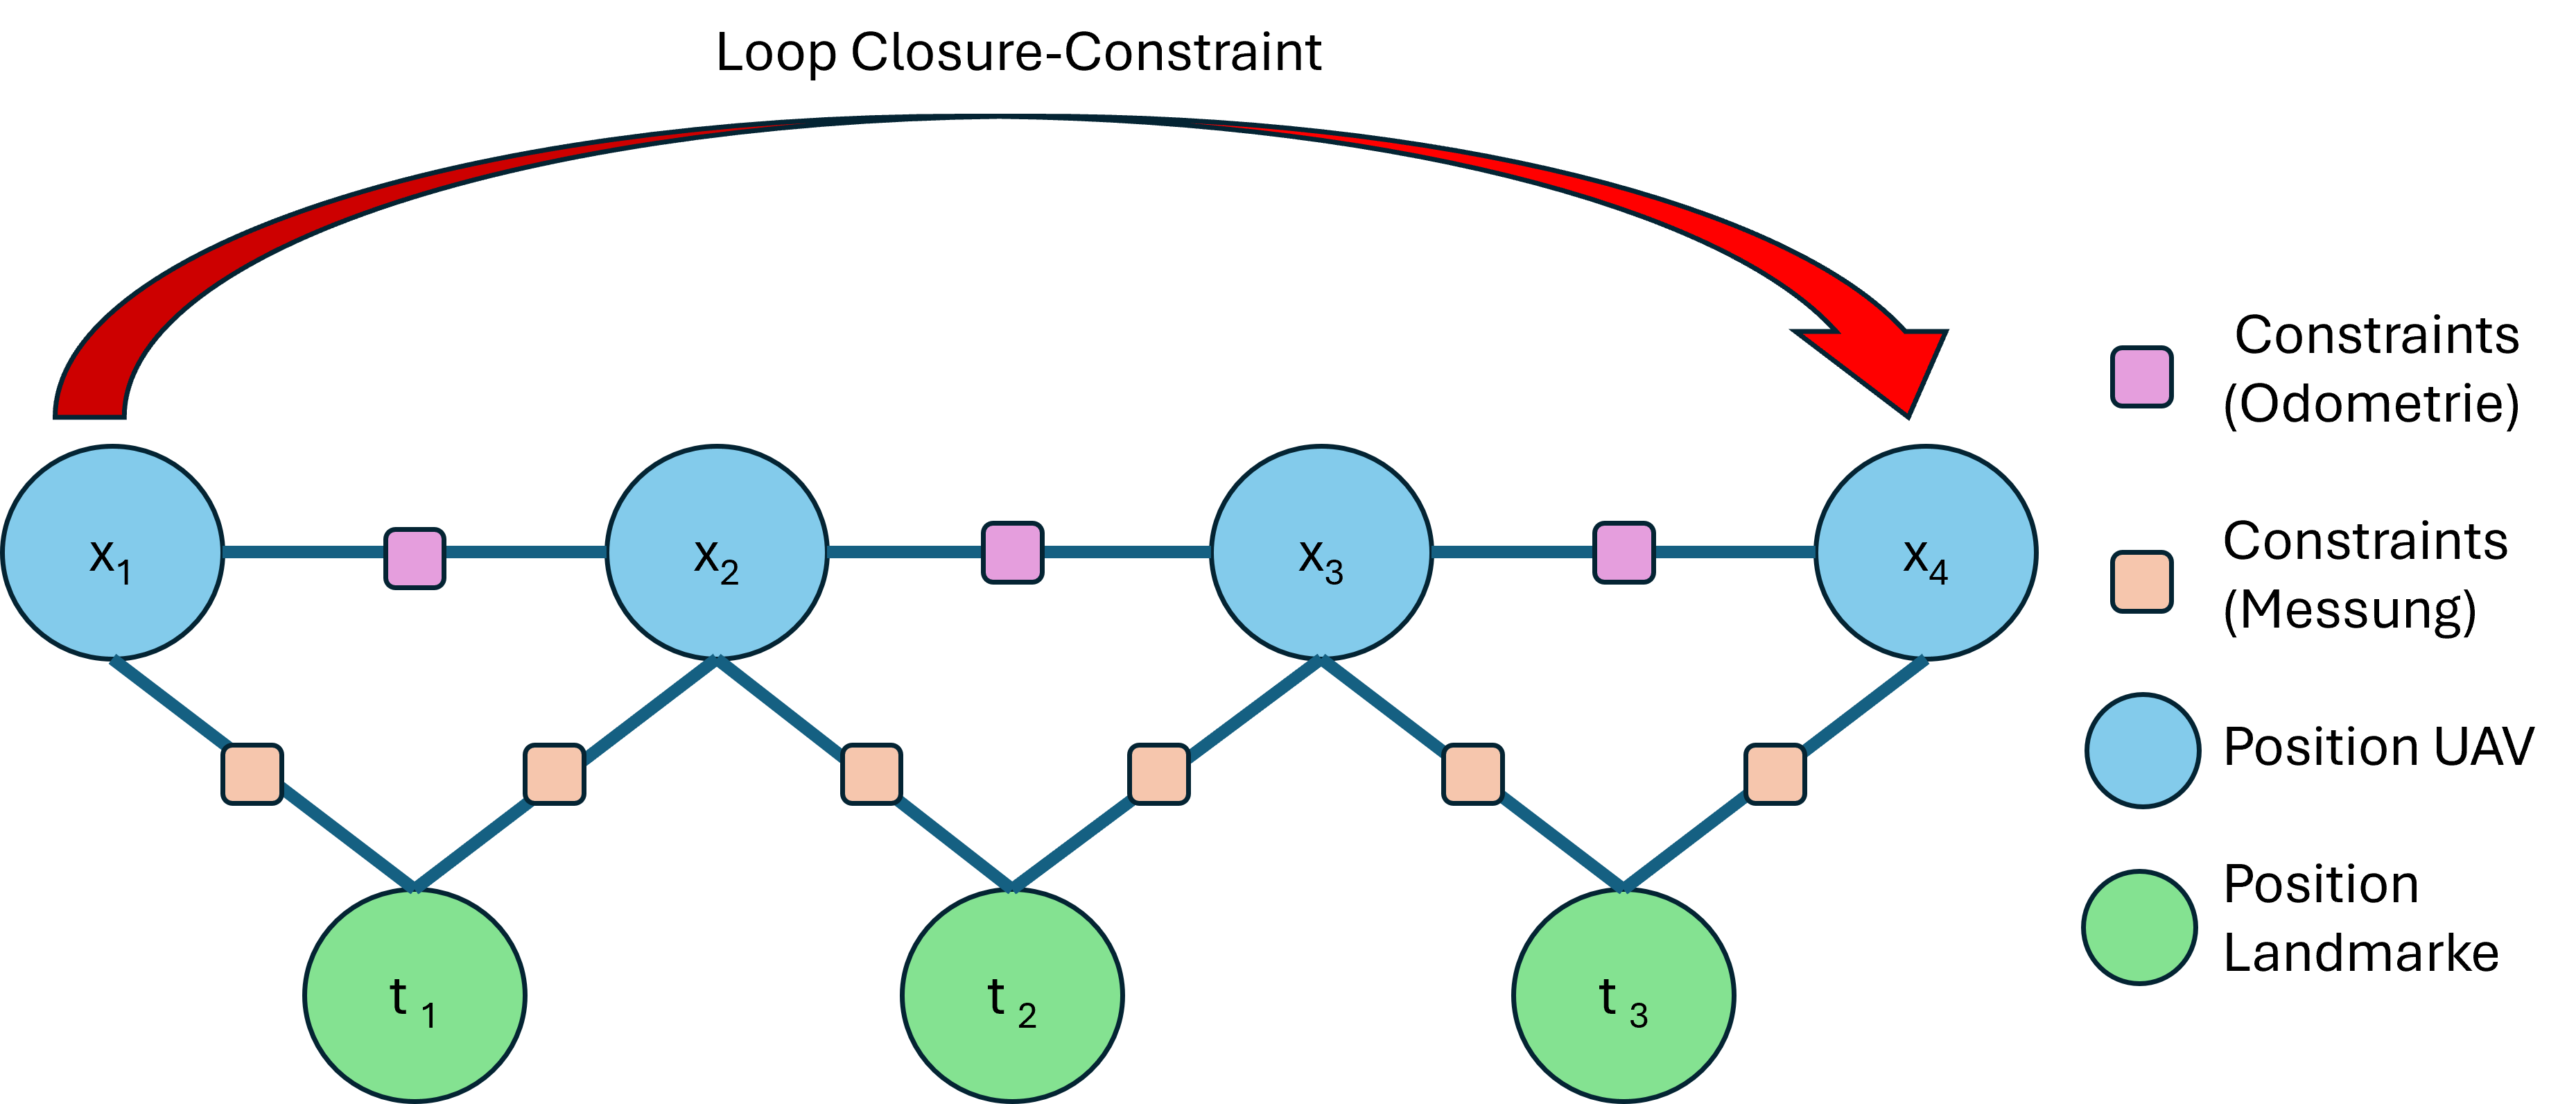
\includegraphics[width=1.0\textwidth]{Bilder/Faktorgraph_vereinfacht.png}
    \caption{Vereinfachter Faktorgraph eines \gls{slam}-Problems, 
    vgl.~\cite{Lai2022}, \cite{Dellaert2017}, \cite{Cai2024}}
    \label{fig:Faktorgraph_vereinfacht}
\end{figure}
\FloatBarrier

Das Ziel der Optimierung ist die Maximum-a-posteriori-Schätzung -- also die Konfiguration aller Variablen (Posen und Landmarken) zu finden, die die 
Gesamtwahrscheinlichkeit aller Beobachtungen maximiert. Äquivalent dazu wird der Gesamtfehler über alle Constraints minimiert.\cite{dellaert2012factor}
Bildlich bedeutet das, dass der Optimierer die Variablen solange ``verschiebt'', bis der Gesamtfehler über allen Messungen minimal ist.



\subsubsection{SLAM-Varianten}
\textbf{\gls{vslam}} nutzt visuelle Sensordaten, um gleichzeitig die Pose eines Roboters zu schätzen und eine Karte der Umgebung zu erstellen.\cite{10169695}
Es baut auf den Konzepten der \gls{vo} und \gls{vio} auf und erweitert diese um die Fähigkeit zur globalen Kartenkonsistenz durch Loop Closure.\cite{Cai2024}


\textbf{ORB-SLAM} ist ein weit verbreitetes Open-Source-\gls{vslam}-System, 
das ORB-Merkmale (Oriented FAST and Rotated BRIEF) zur Merkmalserkennung 
verwendet und sowohl Mono-, Stereo- als auch RGB-D-Kameras unterstützt.\cite{10169695}


\textbf{TagSLAM} ist eine Spezialisierung von \gls{vslam} für Fiducial-Marker.
Anstelle natürlicher Bildmerkmale werden AprilTag-Marker als definierte 
Referenzpunkte verwendet.
TagSLAM nutzt den GTSAM-Faktorgrafen-Optimierer als Backend und ermöglicht 
neben vollständigem SLAM auch extrinsische Kamerakalibrierung und 
Posenschätzung.\cite{TagSLAM}
In dieser Arbeit wird TagSLAM zur Offline-Kartierung der Versuchsumgebung 
eingesetzt.





\section{Fiducial-Marker-Systeme}


\section{Mustererkennung mit RANSAC}



%!TeX root=20_Hauptteil.tex

\chapter{Systembeschreibung}

In diesem Kapitel wird die Testumgebung beschrieben, sowie auf die Softwarearchitekturen eingegangen.
Außerdem wird die Systempipeline erläutert, die zur Entwicklung der Echtzeiterkennung verwendet wurde. 
Es werden die verschiedenen Konzepte vorgestellt, die zur Auswahl eines Echtzeitmodells geführt haben. 



\section{Aufbau der Testumgebung}



\section{Softwarearchitektur}



\section{Systempipeline}


\subsection{elektrischer Aufbau der Holybro X650 mit Pixhawk 6X}

%!TeX root=20_Hauptteil.tex

\chapter{Implementierung der Echtzeiterkennung}



\section{Datensatz- und Objektauswahl}




\section{Training der Modelle}

\subsection{Yolov8 Training}



















%!TeX root=20_Hauptteil.tex

\chapter{Ansteuerung des KUKA iiwa 7 R800}

\section{Kommunikationsschnittstellen}

\section{Greifpunktberechnung}

\subsection{Vortrainiertes Modell Dexnet}

\subsection{Segmentierung mithilfe der Bounding Boxen und dbscan}

\subsection{Segmentierungslogik je Objekt}

%!TeX root=20_Hauptteil.tex

\chapter{Systemintegration}

\section{Gesamtintegration von Echtzeiterkennung, Greifpunktberechnung und Robotersteuerung}

\section{Entwicklung eines Debugging- und Visualisierungsinterfaces}

\subsection{Definieren von Ablageslots}


\section{Analyse des Echtzeitverhaltens}

%!TeX root=20_Hauptteil.tex

\chapter{Test}

\section{Test2}

%!TeX root=20_Hauptteil.tex

\chapter{Zusammenfassung und Ausblick}
\label{cap:zusammenfassung}
Ziel dieser Arbeit war es, ein \gls{uav} zu entwickeln, das sich ohne Satellitennavigation im Innenraum selbst lokalisiert und positioniert.
Die dafür benötigte Positionsschätzung sollte extern berechnet und dem Flugcontroller als Referenz bereitgestellt werden.
Darüber hinaus war ein Verfahren zu bestimmen, das eine unbekannte Umgebung vollständig erfasst oder eine bestehende Karte 
ergänzt und deren Ergebnis der Positionsbestimmung zuführt.

Als Positionsreferenz dienen AprilTags der Familie \texttt{tag36h11}, die auf bedruckter Klebefolie am Boden der Versuchsumgebung ausgebracht sind.
Die Karte umfasst 97 Fiducial-Marker in vier Größen auf einer Fläche von 5,0~m~$\times$~3,9~m.
Ihr Entwurf berücksichtigt, dass ab einer Mindestflughöhe von 1~m stets ausreichend Fiducial-Marker im Sichtfeld der Bodenkamera liegen 
und sieht im Zentrum einen eigenen kleineren Startmarker vor.

Zur Kartierung wurde eine Verarbeitungskette aus Bildaufnahme, Entzerrung, Offline-Detektion der Fiducial-Marker und anschließender Optimierung mit Tag\gls{slam} umgesetzt.
Die Auswahl des Verfahrens erfolgte über eine Nutzwertanalyse der betrachteten \gls{slam}-Varianten.
Die Kartierung läuft offline auf einem externen Rechner und erzeugt aus einer handgeführten Kameraaufnahme eine konsistente Karte aller Fiducial-Marker.
Erprobt wurden drei Parametrierungen, deren Ergebnisse mit einer aus der Druckvorlage abgeleiteten Referenz verglichen wurden.
Der mittlere räumliche Abstand der Fiducial-Markerzentren zur Referenz liegt zwischen 9,57~mm und 12,75~mm.

Für die Positionsbestimmung im Flug wurde ein Node entwickelt.
Er berechnet aus den Detektionen jeder Kamera je Fiducial-Marker eine Kamerapose in der Karte, verwirft widersprüchliche Schätzungen über eine Ausreißerfilterung nach dem \gls{ransac}-Algorithmus und fusioniert die verbleibende Konsensmenge gewichtet.
Die Gewichtung berücksichtigt dabei sowohl die Fiducial-Markergröße und den Abstand als auch die Güte der Karte am Ort des jeweiligen Fiducial-Markers.
Anschließend werden die Kameraposen über die zuvor bestimmte extrinsische Kalibrierung auf den Mittelpunkt des \gls{uav}s transformiert, zeitlich geglättet und in die von \gls{px4} benötigte \gls{ned}/\gls{frd}-Konvention überführt.
Die Übergabe an die Flugsteuerung erfolgt über \gls{uxrce} mit einer Rate von 50~Hz.
Die rechenintensiven Schritte der Entzerrung und der Fiducial-Markerdetektion laufen über Isaac~ROS hardwarebeschleunigt auf dem Begleitrechner.

Der Zustandsschätzer des Flugcontrollers wurde so parametriert, dass er die eingespeiste Pose in Position und Gierwinkel als Stützgröße nutzt, während Satellitennavigation und Magnetometer von der Fusion ausgeschlossen sind.
Zur Flugführung wurde zusätzlich eine Bedienkonsole entwickelt, die Sollpositionen im Kartenkoordinatensystem vorgibt, den Systemzustand anzeigt und einen autonomen Demo-Modus bereitstellt.

Die Erprobung des Gesamtsystems erfolgte in drei Flugversuchen in der Flughalle des \gls{oic}.
Alle Versuche durchliefen den Ablauf aus Steigflug, Schwebeflug, autonomem Abfliegen eines Quadrats und Landung vollständig und ohne Eingriff über die Fernsteuerung.
Die Auswertung der Protokolldateien zeigt, dass der Zustandsschätzer die eingespeiste Pose ohne erkennbare Verzerrung übernimmt und die gestützte Navigation zu keinem Zeitpunkt verlässt.

Die Zielsetzung der Arbeit ist damit erreicht.
Das entwickelte System bestimmt die Pose des \gls{uav}s im Flug allein aus Fiducial-Markerdetektionen und einer vorab erstellten Karte.
Die Karte wird der Flugsteuerung als externe Referenz bereitgestellt.
Ein autonomer Flug innerhalb des kartierten Bereichs ist ohne Satellitennavigation möglich.
Sämtliche Anforderungen aus Abschnitt~\ref{sec:anforderungen} werden erfüllt, wobei die hardwarebeschleunigte Verarbeitung an die eingesetzte Jetson-Plattform gebunden bleibt.

Zugleich bestehen klare Grenzen des Systems.
Ohne eine unabhängige Referenz der wahren Pose lässt sich die absolute Genauigkeit der Positionsbestimmung nicht quantifizieren, sodass die Bewertung des Flugbetriebs auf der Konsistenz der Fusion und dem erfolgreichen Durchlaufen des Versuchsablaufs beruht.
Der nutzbare Flugraum ist auf den Bereich über der Karte und auf einen Höhenbereich beschränkt, in dem die Fiducial-Marker weder zu klein noch außerhalb des Sichtfelds liegen.
Der mit dem Abstand zum Ursprung wachsende Kartenfehler begrenzt zudem die Ausdehnung, bis zu der sich eine Karte ohne zusätzliche Stützstellen sinnvoll erzeugen lässt.

Aus diesen Grenzen ergeben sich mehrere Ansatzpunkte für weiterführende Arbeiten.
Naheliegend ist, den Positionierungs-Node um eine Schätzung der Kovarianz zu erweitern und diese in der ausgegebenen Nachricht mitzuführen.
Der Zustandsschätzer könnte die Vision-Stützung dann anhand der je Nachricht übergebenen Unsicherheit gewichten, statt für jede Messung dieselbe Standardabweichung anzusetzen.
Schätzungen aus wenigen, weit entfernten oder ungünstig erfassten Fiducial-Markern gingen damit schwächer in die Fusion ein als solche aus mehreren gut sichtbaren Fiducial-Markern.

Für die Kartierung empfiehlt sich das Vorgeben vermessener Referenzen etwa alle zwei bis drei Meter.
Solche Stützstellen begrenzen die Strecke, über die sich der Positionsfehler gegenüber dem Ursprung aufbauen kann und ermöglichen damit die Kartierung größerer Umgebungen bei gleichbleibender Genauigkeit.

Der nutzbare Flugraum lässt sich durch eine Erweiterung der Karte vergrößern.
Werden Fiducial-Marker zusätzlich an den Hallenwänden angebracht, kann die bislang ausgeschlossene Frontkamera in die Fusion einbezogen werden.

Ein weiterführender Ansatz besteht darin, die Lokalisierung um weiter Sensoren zu erweitern.
Verfahren der visuell-inertialen Odometrie oder ein \gls{lidar}-gestütztes \gls{slam} bestimmen die Pose aus der natürlichen Struktur der Umgebung und benötigen keine vorab ausgebrachten Fiducial-Marker.
In Verbindung mit der bestehenden Fiducial-Markerkarte ließe sich beides kombinieren, indem die Fiducial-Marker als absolute und driftfreie Stützstellen dienen, während das kartenunabhängige Verfahren den Flug außerhalb des markierten Bereichs trägt.
Damit wäre der Betrieb nicht länger auf die kartierte Fläche beschränkt. Voraussetzung hierfür ist die Funktionstüchtigkeit in der Versuchsumgebung.

Langfristig bildet die entwickelte Positionsreferenz die Grundlage für weiterführende autonome Funktionen im Innenraum.
Mit einer fortlaufend verfügbaren Pose im Kartenkoordinatensystem lassen sich Flugaufgaben planen und wiederholbar ausführen.


% -------------------------------------------------
% Verzeichnisse am Ende
% Einheitlicher Abstand nach den Überschriften
% -------------------------------------------------

% Literaturverzeichnis
\printbibliography


\begingroup
\RedeclareSectionCommand[
  afterskip=0.4\baselineskip
]{chapter}

% Abbildungsverzeichnis
\listoffigures

% Tabellenverzeichnis
\listoftables

% Quellcodeverzeichnis
\renewcommand*{\lstlistlistingname}{Quellcodeverzeichnis}
\lstlistoflistings

\endgroup



% Anhang einbinden
%!TeX root=00_Abschlussarbeit.tex

\chapter{Anhang}
\noindent
Der Anhang enthält ergänzende Informationen, die für das Verständnis der Arbeit relevant sind, aber nicht direkt in den Haupttext integriert werden konnten. 
Dazu gehören beispielsweise ausführliche Tabellen, zusätzliche Abbildungen oder Quellcode, der für die Implementierung der beschriebenen Methoden verwendet wurde.
% \section{Code}
% Anhang mit Quellcode
%\lstset{language=C++,
%                basicstyle=\ttfamily,
%                keywordstyle=\color{blue}\ttfamily,
%                stringstyle=\color{red}\ttfamily,
%                commentstyle=\color{green}\ttfamily,
%                morecomment=[l][\color{magenta}]{\#}
%}

% \begin{lstlisting}[caption={[For-Schleife] For-Schleife die die Zahlen von 1 bis 10 ausgiebt}]
% // Print numbers from 1 to 10
% #include <stdio.h>
% int main() {
%   int i;
%   for (i = 1; i < 11; ++i)
%   {
%     printf("%d ", i);
%   }
%   return 0;
% }
% \end{lstlisting}

\end{document}